\documentclass[10pt,a4,]{article}
% \RequirePackage[l2tabu, orthodox]{nag}
\usepackage[a4paper,text={16.5cm,25.2cm},centering,margin=2.6cm]{geometry}
% \usepackage[left=1.0in,top=1.0in,right=1.0in,bottom=1.0in]{geometry}
\newcommand*{\authorfont}{\fontfamily{phv}\selectfont}
\usepackage{hyperref,amsmath,amssymb,bm,url,enumitem,dcolumn,upquote,framed,alltt,textgreek,xfrac,fixltx2e}
\usepackage[australian]{babel}
\usepackage[compact,small]{titlesec}
\setlength{\parskip}{1.2ex}
\setlength{\parindent}{0em}

\def\tightlist{}

\usepackage{ifxetex}
\ifxetex
  \usepackage{fontspec}
  \defaultfontfeatures{Ligatures=TeX} % To support LaTeX quoting style
 \defaultfontfeatures{Ligatures=TeX,Numbers={OldStyle}}
 \setmainfont{Minion Pro}
 \setsansfont[Scale=MatchLowercase]{Myriad Pro}
 \setmonofont[Scale=MatchLowercase]{Ubuntu Mono}
\else
  \usepackage[T1]{fontenc}
  \usepackage[utf8]{inputenc}
  \usepackage{lmodern}
  % \usepackage[full]{textcomp} % directly use the degree (and some other) symbol
\fi

% place after fonts; even better typesetting for improved readability:
\graphicspath{ {figure/} }
\usepackage{tabularx} % for 'tabularx' environment and 'X' column type
\usepackage{ragged2e}  % for '\RaggedRight' macro (allows hyphenation)
\usepackage{siunitx}
    \sisetup{%
        detect-mode,
        group-digits            = false,
        input-symbols           = ( ) [ ] - + < > *,
        table-align-text-post   = false,
        round-mode              = places,
        round-precision         = 3
        }
% \usepackage[font={small, sf}, labelfont=bf]{caption} % tweaking the captions
\usepackage[font={small}, labelfont=bf]{caption} % tweaking the captions
\usepackage[color=yellow, textsize=tiny]{todonotes}
\frenchspacing%
% \usepackage[kerning=false,protrusion=true,expansion=true]{microtype}

\usepackage{abstract}
\renewcommand{\abstractname}{} % clear the title
\renewcommand{\absnamepos}{empty} % originally center

\renewenvironment{abstract}
{{%
\setlength{\leftmargin}{0mm}
\setlength{\rightmargin}{\leftmargin}%
}%
\relax}
{\endlist}

\makeatletter
\def\@maketitle{%
\newpage
%  \null
%  \vskip 2em%
%  \begin{center}%
\let \footnote \thanks
 {\fontsize{18}{20}\selectfont\raggedright  \setlength{\parindent}{0pt} \@title \par}%
}
%\fi
\makeatother


\setcounter{secnumdepth}{0}





\usepackage{longtable,booktabs}
\setlength\heavyrulewidth{0.1em}
\setlength\lightrulewidth{0.0625em}

\usepackage{graphicx}
% We will generate all images so they have a width \maxwidth. This means
% that they will get their normal width if they fit onto the page, but
% are scaled down if they would overflow the margins.
\makeatletter
\def\maxwidth{\ifdim\Gin@nat@width>\linewidth\linewidth
\else\Gin@nat@width\fi}
\makeatother
\let\Oldincludegraphics\includegraphics
\renewcommand{\includegraphics}[1]{\Oldincludegraphics[width=\maxwidth]{#1}}

\title{The shape of kelp: environmental influences on kelp morphology  }

\author{\Large Ross Coppin\vspace{0.05in} \newline\normalsize\emph{University of the Western Cape}  }

\date{}

% PENALTIES
\widowpenalty=1000
\clubpenalty=1000
\doublehyphendemerits=9999 % Almost no consecutive line hyphens
\brokenpenalty=10000 % No broken words across columns/pages
\interfootnotelinepenalty=9999 % Almost never break footnotes

% SECTION, SUBSECETC.TITLES
\usepackage[compact]{titlesec}
\titleformat{\chapter}
  {\normalfont\LARGE\sffamily\bfseries}
  {\thechapter}
  {1em}
  {}
\titleformat{\section}
  {\normalfont\LARGE\sffamily\bfseries}
  {\thesection}
  {1em}
  {}
\titleformat{\subsection}
  {\normalfont\Large\sffamily\bfseries}
  {\thesubsection}
  {1em}
  {}
\titleformat{\subsubsection}
  {\normalfont\large\sffamily\bfseries\slshape}
  {\thesubsubsection}
  {1em}
  {}
% \titlespacing*{<command>}{<left>}{<before-sep>}{<after-sep>}
\titlespacing*{\chapter}
  {0pt}
  {1.2ex plus 1ex minus .2ex}
  {0.5ex plus .1ex minus .1ex}
\titlespacing*{\section}
  {0pt}
  {1.2ex plus 1ex minus .2ex}
  {0.5ex plus .1ex minus .1ex}
\titlespacing*{\subsection}
  {0pt}
  {1.2ex plus 1ex minus .2ex}
  {0.5ex plus .1ex minus .1ex}
\titlespacing*{\subsubsection}
  {0pt}
  {1.2ex plus 1ex minus .2ex}
  {0.5ex plus .1ex minus .1ex}



\newtheorem{hypothesis}{Hypothesis}
\usepackage{setspace}

\makeatletter

\@ifpackageloaded{hyperref}{}{%
\ifxetex
  \usepackage[setpagesize=false, % page size defined by xetex
              unicode=false, % unicode breaks when used with xetex
              xetex]{hyperref}
\else
  \usepackage[colorlinks=true, citecolor=blue, linkcolor=cyan, pdfborder={0 0 0 }, unicode=true]{hyperref} % place after other packages, but before cleveref
\fi
}

\@ifpackageloaded{color}{
    \PassOptionsToPackage{usenames,dvipsnames}{color}
}{%
    \usepackage[usenames,dvipsnames]{color}
}

\usepackage{cleveref} % cleverly cross referencing figures and tables; last package to include
\setcounter{secnumdepth}{2}
\setcounter{tocdepth}{2}

% To use for resetting the numbering of Appendix Tables and Figures:
%\setcounter{table}{0}
%\renewcommand{\thetable}{A\arabic{table}}
%\setcounter{figure}{0}
%\renewcommand{\thefigure}{A\arabic{figure}}

\makeatother
\hypersetup{breaklinks=true,
            bookmarks=true,
            pdfauthor={Ross Coppin (University of the Western Cape)},
             pdfkeywords = {},
            pdftitle={The shape of kelp: environmental influences on kelp morphology},
            colorlinks=true,
            citecolor=blue,
            urlcolor=blue,
            linkcolor=magenta,
            pdfborder={0 0 0}}
\urlstyle{same}  % don't use monospace font for urls


\begin{document}

% \maketitle

{% \usefont{T1}{pnc}{m}{n}
\setlength{\parindent}{0pt}
\thispagestyle{plain}
{\fontsize{18}{20}\selectfont\raggedright
\maketitle  % title \par
}
{
   \vskip 13.5pt\relax \normalsize\fontsize{11}{12}
\textbf{\authorfont Ross Coppin} \hskip 15pt \emph{\small University of the Western Cape}   
}
}



\vskip 6.5pt

\noindent 

\newpage

\hypertarget{introduction}{%
\subsection{Introduction}\label{introduction}}

Kelps are a group of large seaweeds of the order Laminariales
(Ochrophyta), which despite their relatively low taxonomic diversity of
species in genera (Bolton 2010), nevertheless form the basis of one of
the most productive ecosystems globally (Mann 1973). Kelps generally
have a dependence on cool, temperate and arctic seawater temperatures
(Santelices 2007, Bolton 2010), and dominate the nearshore biomass
within the rocky shallow coasts in both hemispheres (Steneck et al.
2002). Outside of these latitudes, they are also found in cool, deep
water towards the tropics (Graham et al. 2007): this deeper tropical
water, due to its water clarity, also allows for suitable photon flux
and a nitrate concentration (Zimmerman and Kremer 1984, Lüning 1990,
Dayton et al. 1999), the two other environmental variables that support
kelp productivity. Although kelps have a low taxonomic diversity, their
size and complex morphology provide a heterogeneous habitat structure
(Steneck et al. 2002) that accommodate a multitude other turf and
subcanopy seaweed species, and diverse assemblages of sessile and mobile
invertebrates and vertebrates ({\textbf{???}}, Mann 1973, Steneck et al.
2002), each depending on a wide suite of ecological services provided by
the kelp and the habitat structure they provide (Gaines and Roughgarden
1987, Bologna and Steneck 1993, Levin 1994, Anderson et al. 1997).

\hypertarget{background}{%
\subsubsection{Background}\label{background}}

Kelps are sessile species and have to adapt to local environmental
conditions in order to grow, repruce and persist. The resilience of
kelps is evident through their distribution, which spans a range of
environmental conditions that vary spatially and temporally. Wave
exposure and temperature are regarded as important environmental drivers
with regards to macroalgae, and play a role in the distribution,
abundance, diversity, composition, growth (Cousens 1982) and
productivity (Pedersen and Nejrup 2012) of kelps. Wave exposure is
recognised as the main cause of kelp mortality, which may manifest
itself through dislodgment of individuals or breakage of important
morphological structures. These mechanisms usually occur during times of
high wave energy or pulse disturbance events, such as storms. Mechanical
forces generated by the hydrodynamic environment, in the form of sudden
strong ocean currents or storms, between 10-20 m.s\textsuperscript{-1}
with accelerations of 400 m.s\textsuperscript{-1} (Friedland and Denny
1995) are the biggest threat to kelp survival. Kelps are able to reduce
the probability of dislodgment or breakage through morphological
adaptation, which may involve several strategies. Kelps can either
reduce drag, increase attachment strength, or increase flexibility in
order to survive high wave energy environments. The strategy that the
algal organism employs is dependent on the species. For instance,
branched, articulated algae will vary its morphology differently to that
of foliose, more flexible macroalgae. Moss (1948) investigated the
anatomy and chemical composition of \emph{Fucus spiralis} at three sites
that varied in wave exposure (sheltered, medium exposure and exposed).
The author found that individuals in exposed sites showed less branching
of thalli as well as variation physiological components, such as organic
nitrogen, mannitol, laminarian and alginic acid concentrations. The
authors also noted a `crumpling effect' displayed by individuals from
exposed sites and inferred that this strategy may reduce overall drag.
Other studies show that macroalgae in wave exposed environments have
morphologies that reduce overall drag, increase strength of attachment
or increase flexibility. For example, a study by Fowler-Walker et al.
(2006) looked for differences in morphology of \emph{Ecklonia radiata}
between wave-sheltered and wave-exposed sites, using a combination of
\emph{in situ} sampling and transplantation of juvenile plants. The
results showed that morphology differed between wave-sheltered and
wave-exposed sites, with thin thalli developing at sheltered sites and a
narrower, thicker thallus with a thick stipe forming at exposed sites.
This finding was consistent with previous studies \{AJS: name the
studies and the species involved here\}. Juveniles transplanted into
wave exposed sites underwent rapid morphological adaptation, whilst the
opposite was true for wave-sheltered sites, which showed slower
morphological adjustment \{refs.\}. Dislodgement through increased wave
exposure is not the only hydrological variable playing a role in kelp
mortality. A study by Bettignies et al. (2013) tested if there is a link
between orbital water velocity representative of wave-swept reefs and
the morphology and biomass of \emph{Ecklonia radiata}. The results
showed that morphological adaptation through drag reduction and strength
increase does not reduce drag as efficiently as reduction in overall
biomass through reduction in thallus surface area. The authors concluded
that at peak orbital water velocities, size (as biomass) and not
morphological adaptation was the main determinant of hydrological
performance in wave-swept environments.

There is also evidence that morphological adaptation is driven by
currents, and in fact may be driving hydrological performance of
macrolgae. Duggins et al. (2003) examined the direct and indirect flow
effects on population dynamics, morphology and biomechanics of several
understorey macroalgae species. These species included \emph{Costaria
costata}, \emph{Agarum fimbriatum}, \emph{Laminaria complanata} and
\emph{Nereocystis luetkeana}. The results showed that wave impacted
sites (wave exposed) exhibited higher rates of mortality, and no
significance was found between survival of individuals and tidal or
current velocity. The authors concluded that although tidal and current
velocity did not play a significant role in determining kelp survival,
it did play a role in morphological adaptation. The results from this
study suggest that high current and tidal stresses are the main driver
of kelp morphological adaptation. This in turn make those individuals
more resilient to dislodgement to wave exposure. Wave exposure is
stochastic in nature compared to tidal and ocean currents which are more
regular in their frequency and magnitude. Therefore the regular forces
of tidal and ocean currents may make kelp individuals more resilient to
mechanical dislodgement over time.

\hypertarget{the-south-african-context}{%
\subsubsection{The South African
context}\label{the-south-african-context}}

The biogeographic distribution of kelp is limited by seawater
temperature (Bolton 2010), where increasing temperature gradients reduce
kelp distribution. Due to this limiting factor, the two main species of
kelps in southern African waters, \emph{Ecklonia maxima} and
\emph{Laminaria pallida}, are distributed along a section of the south
coast from De Hoop, extending west around the Cape Peninsula, and
thriving north into Namibia (Molloy and Bolton 1996, Stegenga et al.
1997). This distribution follows a temperate gradient, where sea
temperatures increase as one moves south from Namibia, around Cape Point
and towards De Hoop. Although the two species occur together for the
majority of the coast, their basic morphologies and resource needs vary
to a degree. The larger species, \emph{Ecklonia maxima}, is distributed
from Lüderitz to Cape Agulhas (Fig. 1) (Bolton and Levitt 1985, Probyn
and McQuaid 1985, Bolton and Anderson 1987, Bolton et al. 2012).

\begin{figure}
\centering
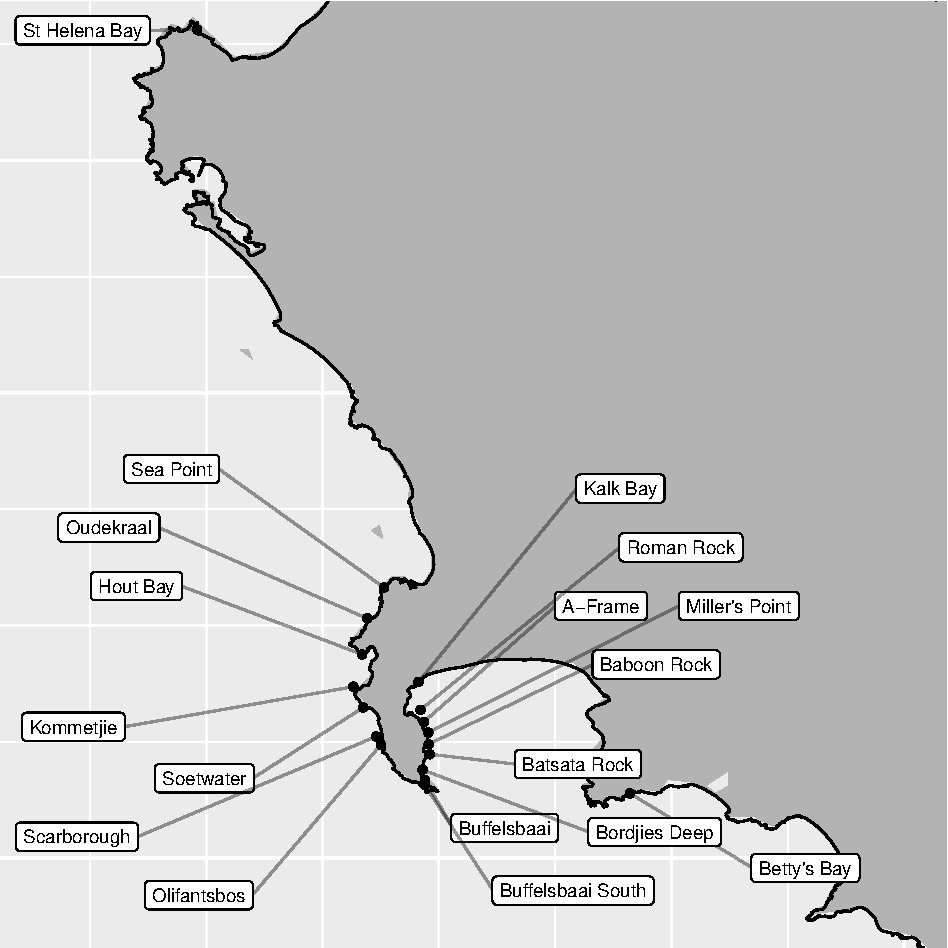
\includegraphics{chapter_2_files/figure-latex/unnamed-chunk-1-1.pdf}
\caption{A map indicating the sites where morphometric measurements were
collected for \emph{Ecklonia maxima} and \emph{Laminaria pallida}.}
\end{figure}

Characterised by a large distal swollen bulb filled with gas, and smooth
fronds, this species grows to approximately 10 meters (Bolton and
Anderson 1987). There was, however, a 17 m specimen collected in 2015
off Cape Point (Smit, unpubl. data). This species of kelp not only
dominate the biomass of the South African nearshore, but plays an
important ecological role (Bustamante and Branch 1996). The estimated
productivity of \emph{Ecklonia maxima} within South Africa varies
between 350 and 1500 gC.m\textsuperscript{-2}yr\textsuperscript{-1}
(Mann 1982). Across the majority of the coastline, \emph{Laminaria
pallida} remains a subsurface kelp, dominating the kelp biomass at
depths greater than 10 m (Field et al. 1980a, Bolton and Anderson 1987,
Molloy and Bolton 1996). This species is distributed from Danger Point,
east of the Cape Peninsula, to Rocky Point in northern Namibia, and
reaches depths of greater than 20 m (Field et al. 1980a, Molloy and
Bolton 1996, Stegenga et al. 1997). Towards the north along the west
coast, from around Hondeklipbaai, \emph{Laminaria pallida} replaces
\emph{Ecklonia maxima} as the dominant kelp species (Velimirov et al.
1977, Stegenga et al. 1997) and it also occupies increasingly shallower
subtidal regions. The northern populations also exhibit an increase in
stipe hollowness, compared to the solid stipe morphs in the species'
southern distributions (Molloy and Bolton 1996). This variation in
morphology was thought to represent two distinct species, with the
northern populations formerly described as \emph{Laminaria schinzii}
Foslie (Molloy and Bolton 1996). Genetic work has subsequently shown
that the two morphs are in fact the same species (Rothman et al. 2017).
In southern African waters, the primary production of \emph{Laminaria
pallida} is between 120 and 1900g C m2yr1, similar to that of
\emph{Ecklonia maxima} (Mann 1982). Primary production is not the only
pathway.

The aim of this study is, therefore, to understand how environmental
drivers such as temperature and wave energy can influence
morphoplasticity in two species of kelps around South Africa. This will
be achieved by initially understanding the variation in abiotic
parameters, and morphometrics of \emph{Ecklonia maxima} and
\emph{Laminaria pallida}, around the Western Cape coast. Thereafter we
will look at how the abiotic parameters both correlate and influence
each other in the nearshore environment of our study region. Finally, we
will investigate which abiotic parameters best describe the
morphological variation of the two kelp species, using statistical
tools. It is predicted that higher wave energy environments will exhibit
kelps with reduced undulations, possessing strap-like blades, opposed to
low flow regimes that will show greater undulations in frond morphology.
An increase in temperature is predicted to influence specific
morphological traits that rely on nutrient uptake, as temperature and
nutrients share an inverse relationship. An increase in temperature is
also predicted to reduce the dominance of the colder water kelp,
\emph{Laminaria pallida}, at depth, with a total absence of
\emph{Laminaria pallida} as one approaches the eastern boundary of
sample sites.

\hypertarget{study-area}{%
\subsubsection{Study area}\label{study-area}}

Due to the Cape Peninsula's temperate latitude, winter months bring an
increased frequency of frontal depressions that originate from the
Southern Ocean (Reason et al. 2006). These low pressures are joined by
large swells with increased wave energy. The nearshore environment, with
the accompanied biota, therefore experiences high wave energy events,
with increased frequency in winter (Veitch et al. 2018). The large
peninsula acts as an obstruction for large south westerly swells,
providing decreased wave energy along the west side of False Bay
(Shipley 1964). Conversely, the west coast of Cape Point is battered by
these large swells at full force. Multiple sites, therefore, exist where
kelps grow in diverse temperature and wave energy climates, in close
proximity.

In Figure 2 the total and seasonal wave roses of the directional wave
buoy just offshore from Cape Town is given form the years 2000 till end
2017 (the period for which directional wave spectra was available). It
is due to the near consistent South-westerly swell waves and the complex
orography around the peninsula, that the wave energy distribution around
the Cape Peninsula varies significantly over a small geographical area.
For details on the seasonality of the wave climate around the Cape
peninsula please refer to (Veitch et al. 2018).

\begin{figure}
\centering
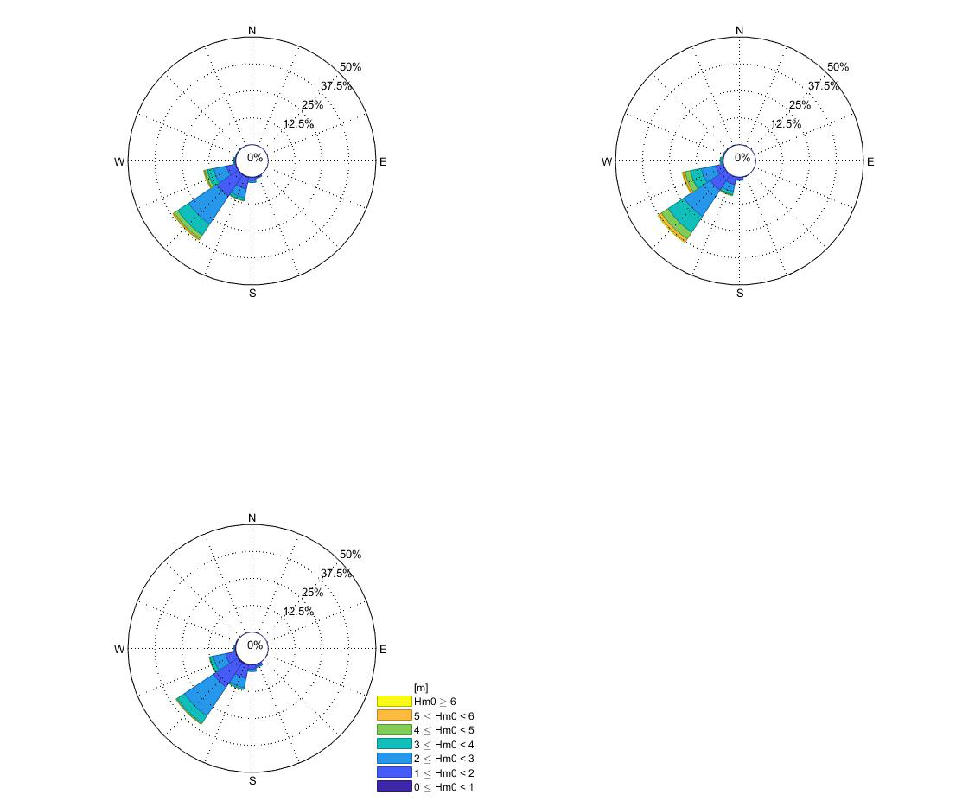
\includegraphics{chapter_2_files/figure-latex/unnamed-chunk-2-1.pdf}
\caption{Wave roses of the Cape Point wave rider buoy situated at
18.29oE, message=FALSE, warning=FALSE, 34.2oS in 70m water depth. (a)
total wave record, (b) winter waves and (c) summer waves.}
\end{figure}

In Figure 3 the total coastal wave exposure of the Cape Peninsula is
given in terms of wave energy (kW per meter wave crest length). These
values have been computed using model output from approximately 20 year
of simulated nearshore wave conditions. Hindcast global wave parameters
were refracted into the nearshore via a spectral phase-averaged
numerical wave modelling code SWAN (Simulating, WAves in the Nearshore -
3rd generation). The model is fully spectral in all frequencies and
directions (0o -360o) (can solve swell and local wind generated waves
simultaneously, propagating in different direction) and was used to
model the propagation of short crested swell waves, waves generated by
wind, non-linear wave-wave interaction and dissipation and depth induced
breaking and refraction. Wave energy dissipation due to bottom friction
and whitecapping is also accounted for ({\textbf{???}}).

Time series output from 1997 till 2013 of this model was then produced
at the 7m and 15m depth contour lines. Each nearshore output point thus
contained a 17-year timeseries of significant wave heights, peak periods
and mean wave directions (with both swell and wind waves). This data set
is available on a 500m resolution around most of the South African
coastline and on a 200m resolution with False Bay as provided by the
South African Department of Environmental Affairs (DEA) and Council for
Scientific and Industrial Research (CSIR)(@Theron2014). The total
17-year average energy, for each output location, was then computed
using linear wave theory, taking into account deep, intermediate and
shallow water wave approximations (based on wave length) for the wave
energy ({\textbf{???}}, {\textbf{???}}, {\textbf{???}}) which is a
function of wave height and period.

The directional sheltering effect of the Cape Peninsula, against the
dominant swell direction, (given in Figure 2) is clear observed in the
wave exposures presented in Figure 2. The classification from fully
sheltered to extremely exposed is based on the total wave energy upper
and lower limits. It should be noted that what is classified as
sheltered around the South African coastline (a high energy coastline)
might be classified as exposed in other regions of the world
({\textbf{???}}, Norderhaug et al. 2012, Sundblad et al. 2014). Kelp and
other ecosystems adapt to their typical environmental exposure and thus
what is classified as extreme abiotic coastal forcings (temperature,
winds, waves and currents) will vary around the world depending on the
geographical setting.

From Figure 2 the western periphery of the Cape peninsula is almost
continuously producing high coastal wave exposures while the Eastern
periphery of the peninsula (western coastline of False Bay) revealed
sheltered wave exposures. Here the marked seasonality, with higher
energy waves during winter, may be clearly observed once more.

\begin{figure}
\centering
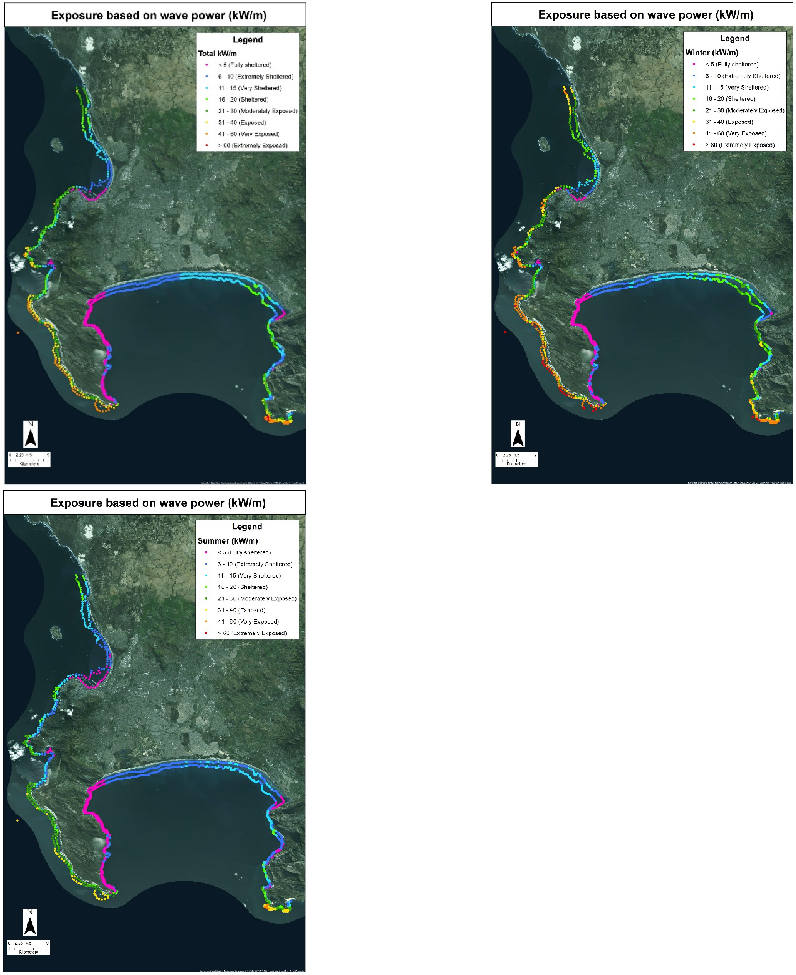
\includegraphics{chapter_2_files/figure-latex/unnamed-chunk-3-1.pdf}
\caption{Coastal wave energy exposure around the Cape Peninsula for the
(a) total 17-year nearshore wave record, (b) only winter months and (c)
only summer months.}
\end{figure}

In Figure 3 the propagation of a typical offshore wave spectrum is given
as produced from a single time-step in SWAN. Figure 3 is presented to
clarify the averaged wave exposure maps presented in Figure 4. Tracing
the wave height contours into False Bay its clear why this Bay's western
periphery is predominantly sheltered. It should be mentioned that some
of the annual winter frontal depression systems pass the Cape Peninsula
from the west to east, resulting in wave propagating towards the
continent from much more southerly directions. This results in positive
and negative wave exposure anomalies all around the peninsula.

\begin{figure}
\centering
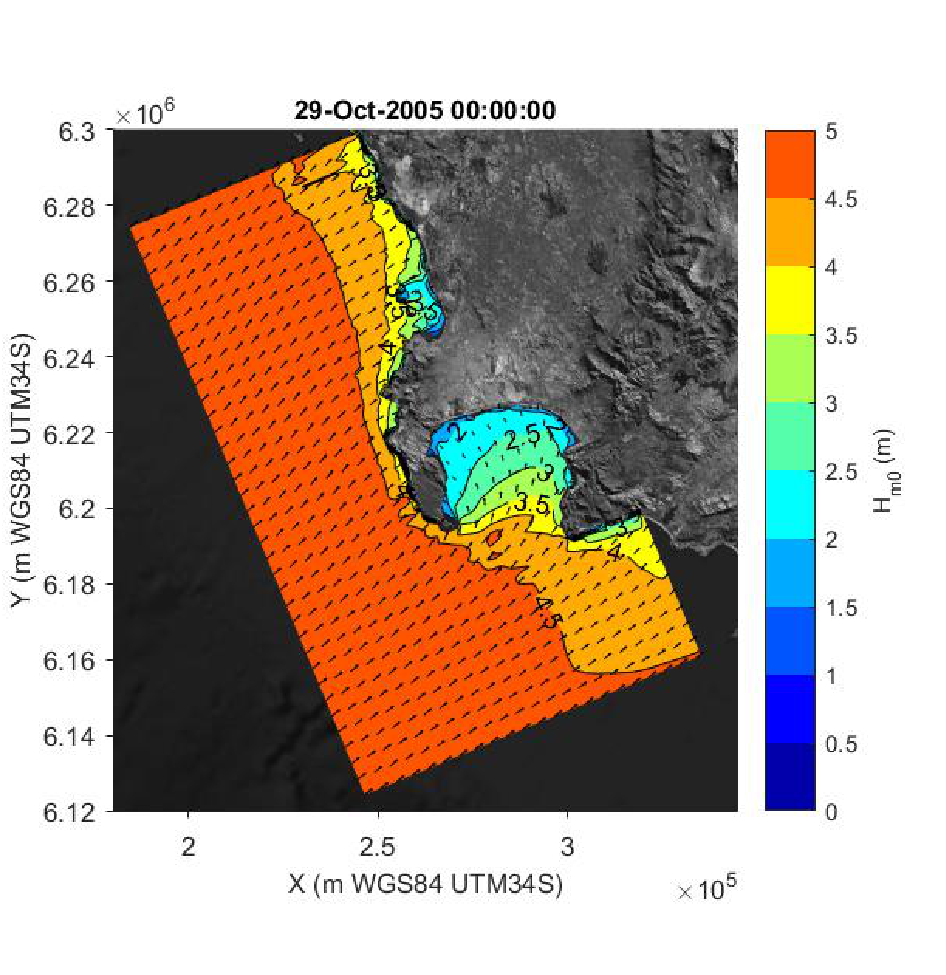
\includegraphics{chapter_2_files/figure-latex/unnamed-chunk-4-1.pdf}
\caption{SWAN numerical output for an example typical offshore wave
conditions refracting around the Cape Peninsula.}
\end{figure}

\newpage

\hypertarget{methods}{%
\subsection{Methods}\label{methods}}

\hypertarget{morphometrics-collection}{%
\subsubsection{Morphometrics
collection}\label{morphometrics-collection}}

Between October 2014 and April 2015, morphological measurements of
\emph{Laminaria pallida} and \emph{Ecklonia maxima} were collected at 18
sites along the Western Cape coast of South Africa (Fig. 1). Eleven
samples were collected per morphology, for each species (Table 1, 2).
These varying morphometrics allowed measurements such as weight, length
and thickness to be compared between sites. Because the macroalgae
differ in morphological features, species-specific morphometrics were
included. These sites span across the majority of the south-west coast,
in varying thermal and wave energy regimes.

Between February 2017 and Novevember 2018, morphological measurements
for \emph{Ecklonia maxima} individuals in shallow water (\textless{}1m)
at 5 sites along the Western Cape coast of South Africa were collected.
These sites represent a wave gradient moving south along the peninsula
and into False Bay. The same morphometric measurements were taken as per
the deeper \emph{Ecklonia maxima}, and this allowed comparison between
morphological characteristics between deep and shallow individuals.

\hypertarget{sites}{%
\subsubsection{Sites}\label{sites}}

Sites were chosen to represent an array of morphological differences
seen within \emph{Ecklonia maxima} and \emph{Laminaria pallida}. Sites
were also chosen to reflect locations that displayed variable wave and
temperature regimes (Fig. 2-5), to allow us to robustly test our
hypothesis of environmental drivers influencing kelp morphology.
St.~Helena Bay and Betty's Bay constituted the north western and south
eastern boundary sites respectively. These sites are roughly 300km
apart, and lie within separate marine provinces, as outlined above. The
Cape Peninsula provides an interesting topographical boundary that
shelters the coast in False Bay. Sites were therefore chosen to
represent an array of environments, from offshore reefs (Batsata Rock),
to sheltered intertidal zones (Miller's Point). West of Cape Point, a
number of sites were chosen to highlight the presence of upwelling
(Oudekraal, Kommetjie), as well as kelps growing in protected bays (Hout
Bay).

\hypertarget{abiotic-parameters}{%
\subsubsection{Abiotic parameters}\label{abiotic-parameters}}

In order to compare abiotic parameters for sites around the coast, large
historical databases for both temperature and wave energy were accessed.
Shallow water temperatures were sourced from the South African Coastal
Temperature Network (SACTN) website
(\url{https://github.com/ajsmit/SACTN}). Seven different organisations
within South Africa contribute to the SACTN, where \emph{in situ}
temperature measurements are made around the South African coast using
either hand-held thermometers or digital temperature recorders
positioned underwater. The mean duration of the 135 daily time series is
19.7 years, and these \emph{in situ} data are preferred over satellite
SST, which have shown to exhibit large biases (Smit et al. 2013). Linear
interpolated SST were calculated for sites where \emph{in situ}
recorders were absent. Wave energy data formed part of the South African
Coastal Vulnerability Assessment, presented to the Department of
Environmental Affairs ({\textbf{???}}). These data are first forecasted
using NOAA Wave Watch III (WWIII), with National Centers for
Environmental Predictions (NCEP) product as the numerical input
({\textbf{???}}). Hindcast data from WWIII span from 1994-2013 at a
3-hour resolution. The data are then used to model short --crested waves
generated by the wind into the coastal environment, using Simulating
Waves in the Nearshore SWAN ({\textbf{???}}). SWAN allows one to extract
wave parameters from specific gridded locations in the nearshore. For
False Bay, a resolution of 200 meters was modelled, at both 7 meter and
15 meter contours. A 200 meter resolution was used as False Bay was
nested within a larger grid area for the research from where the data
were sourced. For Table Bay and east of Cape Hangklip the resolution 500
meters at 7 meters and 15 meters. For this study the 7 meter contours
were used.

\#\#\#Statistical analyses

To compare how kelp morphology varies around the coast, boxplots were
constructed to summarise descriptive statistics for all the
morphometrics of both species.These boxplots highlight five different
descriptive statistics (Minimum, 25\textsuperscript{th} percentile,
median, 75\textsuperscript{th} percentile and maximum), as well as the
interquartile range. These allow us to visually identify variations and
differences in morphology, and to provide evidence that kelp
morphologies vary around the coast.Pairwise correlations were plotted to
compare the abiotic parameters and understand if wave and temperature
parameters correlate with one another around the coast. Therefore
fluctuations such as minimum, maximum, range and standard deviations
were included as temperature parameters, and standard deviations were
included as wave parameters. Median calculations were made for wind and
wave direction, as issues arise when calculating mean and standard
deviation for compass metrics. Redundancy Analyses (RDA) were performed
to understand how kelp morphology is driven by environmental drivers. An
RDA performs multiple linear regressions between explanatory and
response variables. This allows the user to calculate the amount of
variation in response variables explained for by explanatory variables.
Therefore response variables are influenced by explanatory variables.
Response variables were represented by morphology measurements, with
wave and temperature variables selected as explanatory variables.
Temperature and wave parameters were modelled separately, to fully
understand and tease apart which abiotic variables most strongly explain
kelp morphology variation. This was therefore performed for each
species, equating to four RDA's in total.

\newpage

\hypertarget{results}{%
\subsection{Results}\label{results}}

\hypertarget{temperature-parameters}{%
\subsubsection{Temperature parameters}\label{temperature-parameters}}

The temperature parameters around the Western Cape coast vary among
sites and seasons. During February and August, the west side of Cape
Point experiences decreased temperatures (Fig. 5). This region also
experiences lower mean and maximum temperatures when compared to False
Bay, a region known as east of Cape Point. The range of temperatures
within False Bay are larger in winter (August) compared to summer
(February) (Fig. 5). The sites north of Kommetjie on the west side
display larger temperatures ranges than sites south of Kommetjie on the
west side.

\begin{figure}
\centering
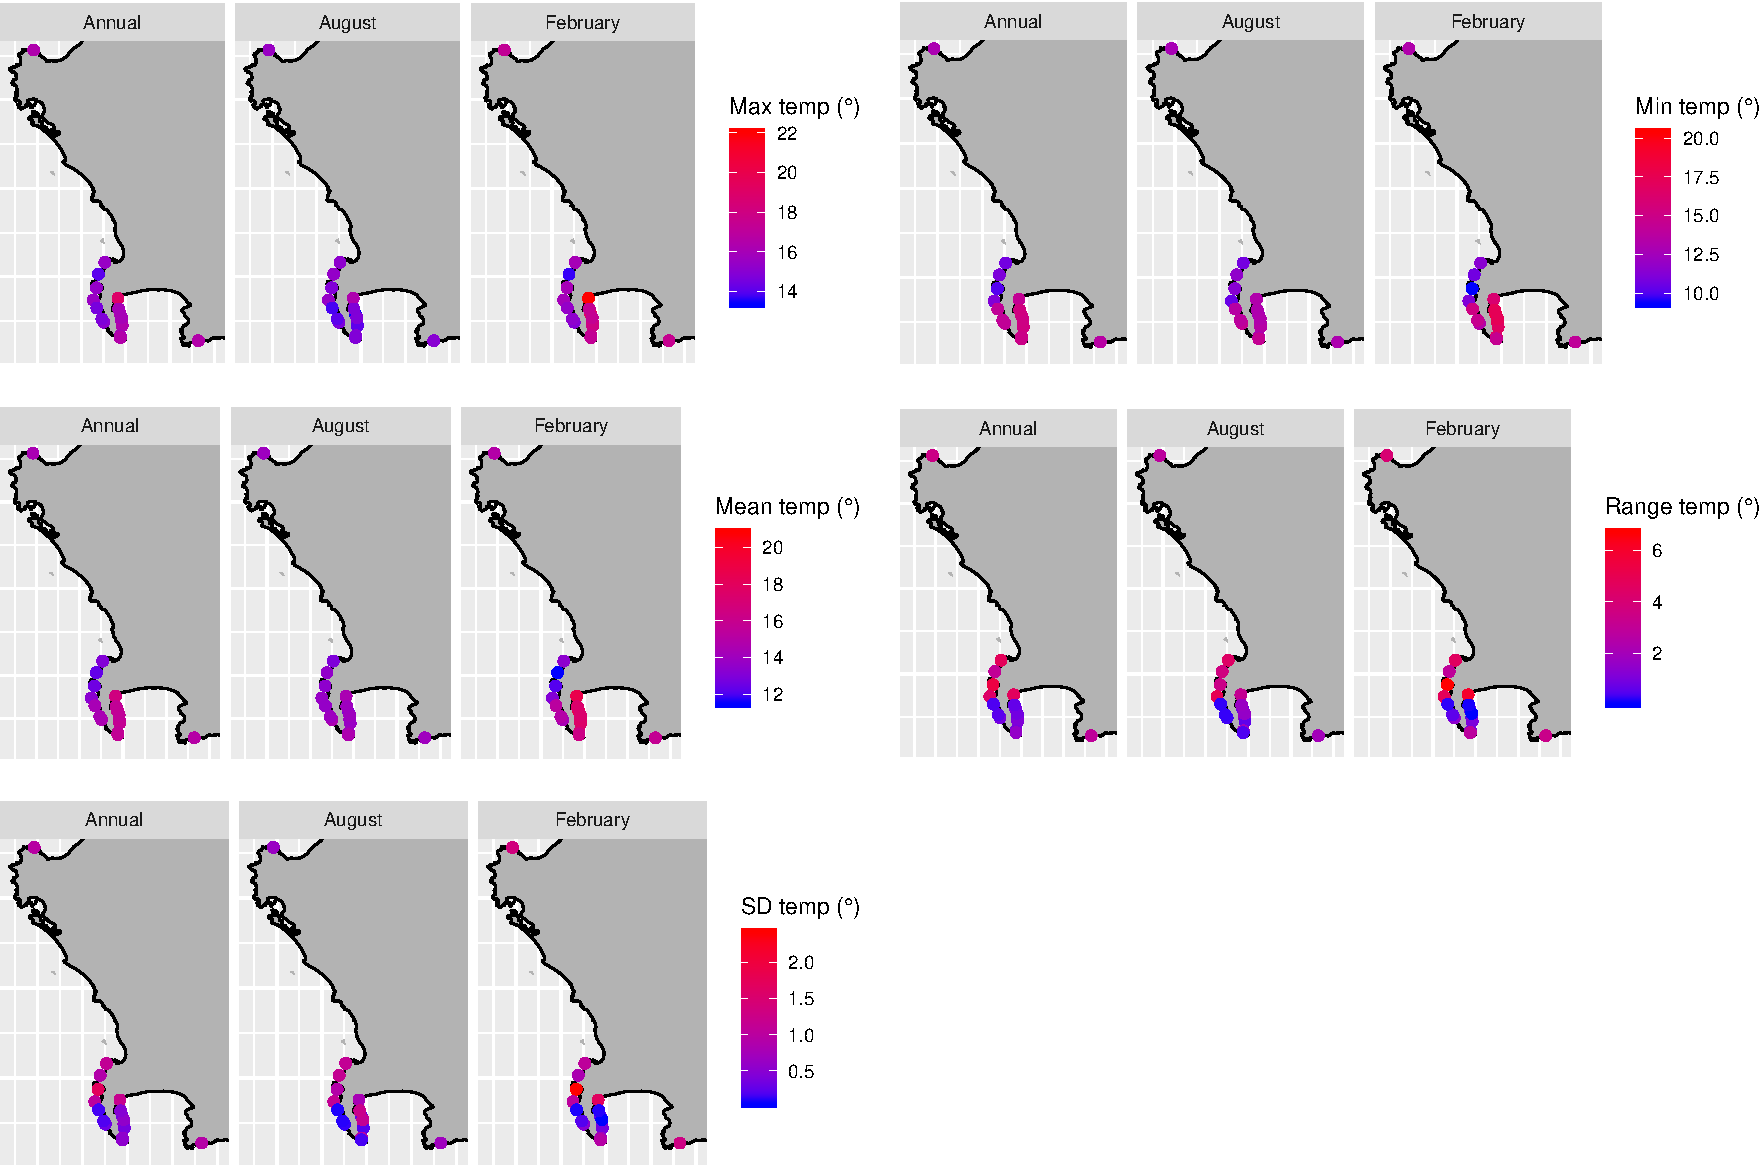
\includegraphics{chapter_2_files/figure-latex/unnamed-chunk-12-1.pdf}
\caption{Temperature parameters relative to each morphometric collection
site around the Western Cape coast. Temperature parameters include
minimum, maximum, mean, range and standard deviation (° Celsius). These
site locations are coloured by the temperature statistic relative to the
legends provided. Each temperature parameter is also divided into August
(winter) and February (summer) as well as the annual mean.}
\end{figure}

\hypertarget{wave-and-wind-parameters}{%
\subsubsection{Wave and wind
parameters}\label{wave-and-wind-parameters}}

Not only do the temperature parameters display seasonal fluctuations,
but we see similar observations for wave parameters. The west side of
Cape Point exhibit increased median direction, SD and mean significant
wave height compared to within False Bay (Fig. 4). Sites within False
Bay however display increased standard deviations of wave period. Median
wind direction is northerly in winter (Fig. 6), and turns southerly in
summer.

\begin{figure}
\centering
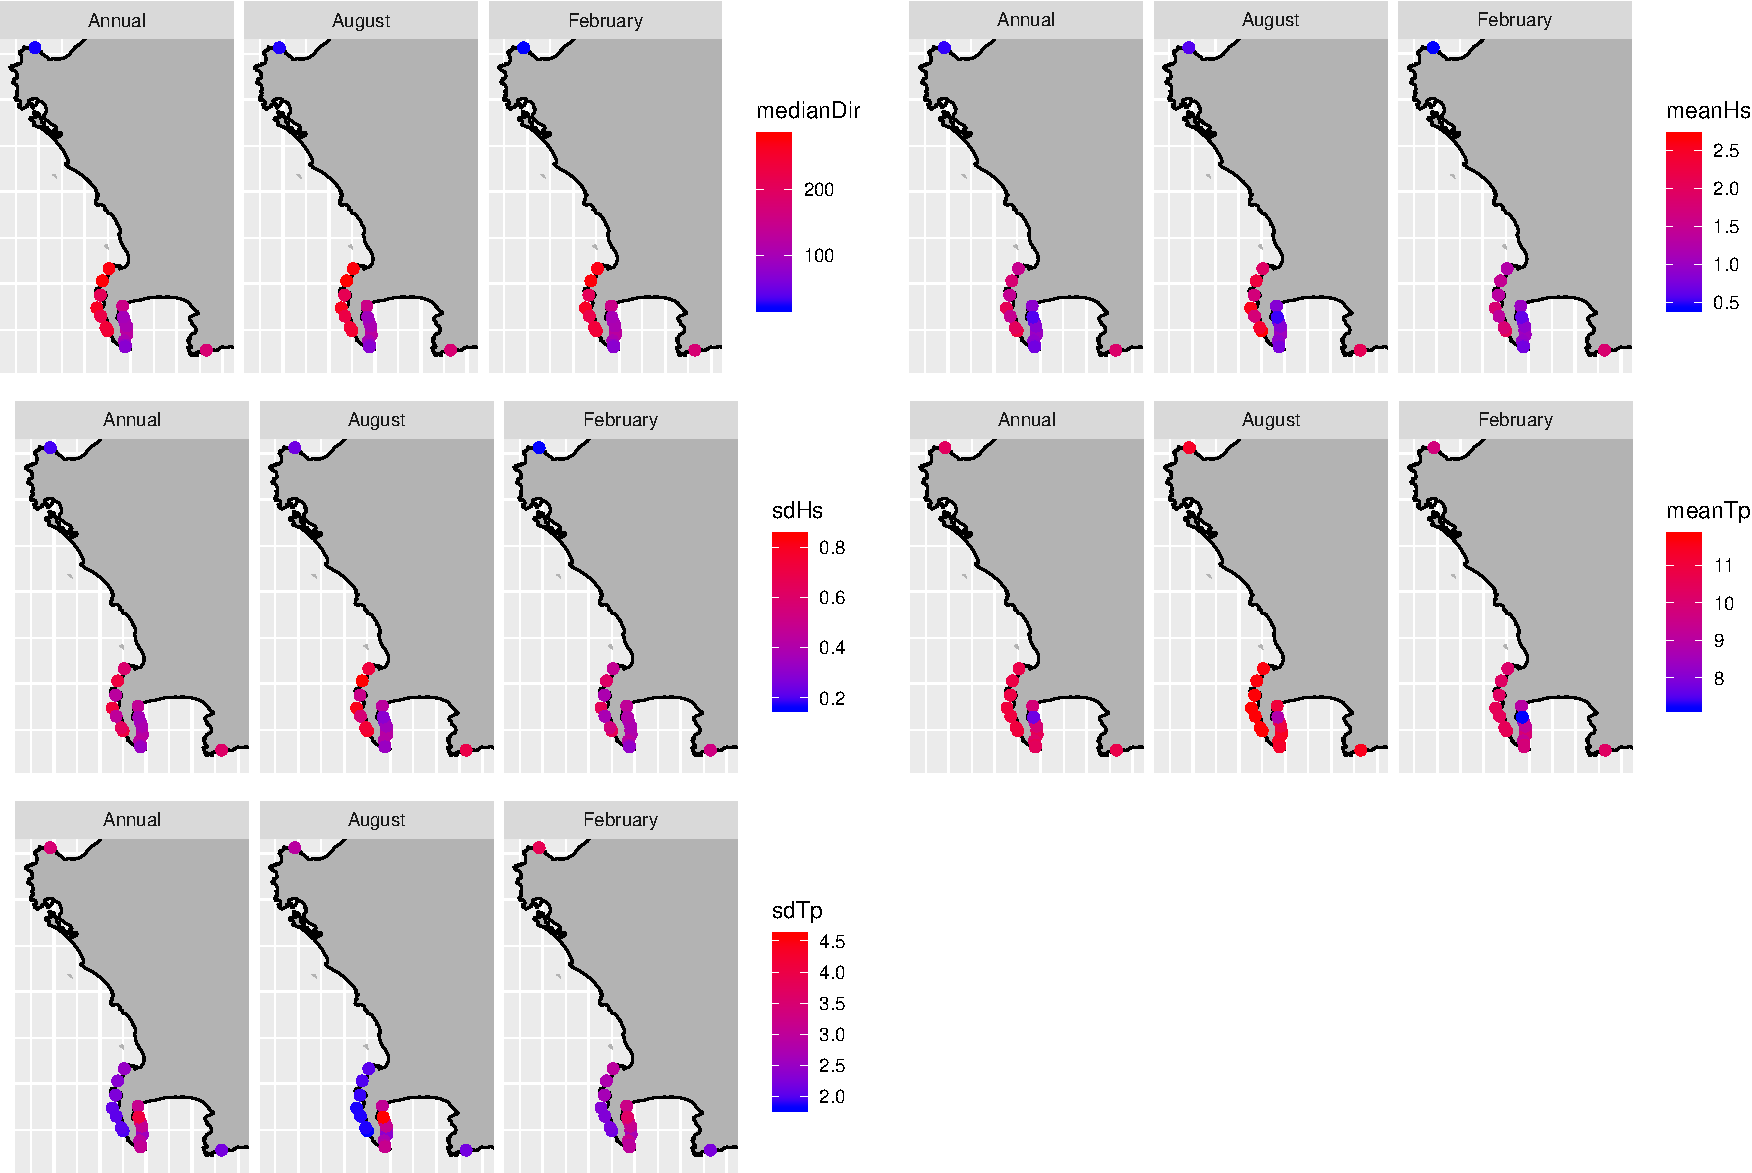
\includegraphics{chapter_2_files/figure-latex/unnamed-chunk-15-1.pdf}
\caption{Wave parameters relative to each morphometric collection site
around the Western Cape coast. These wave parameters include mean and
standard deviation of wave direction (° True north), significant wave
height (Meters) as well as wave period (Seconds). Sites are colour-coded
by the parameter statistic provided by the legend. Each wave parameter
is also divided into August (winter), February (summer) and annual
means, to visualise seasonal differences.}
\end{figure}

\begin{figure}
\centering
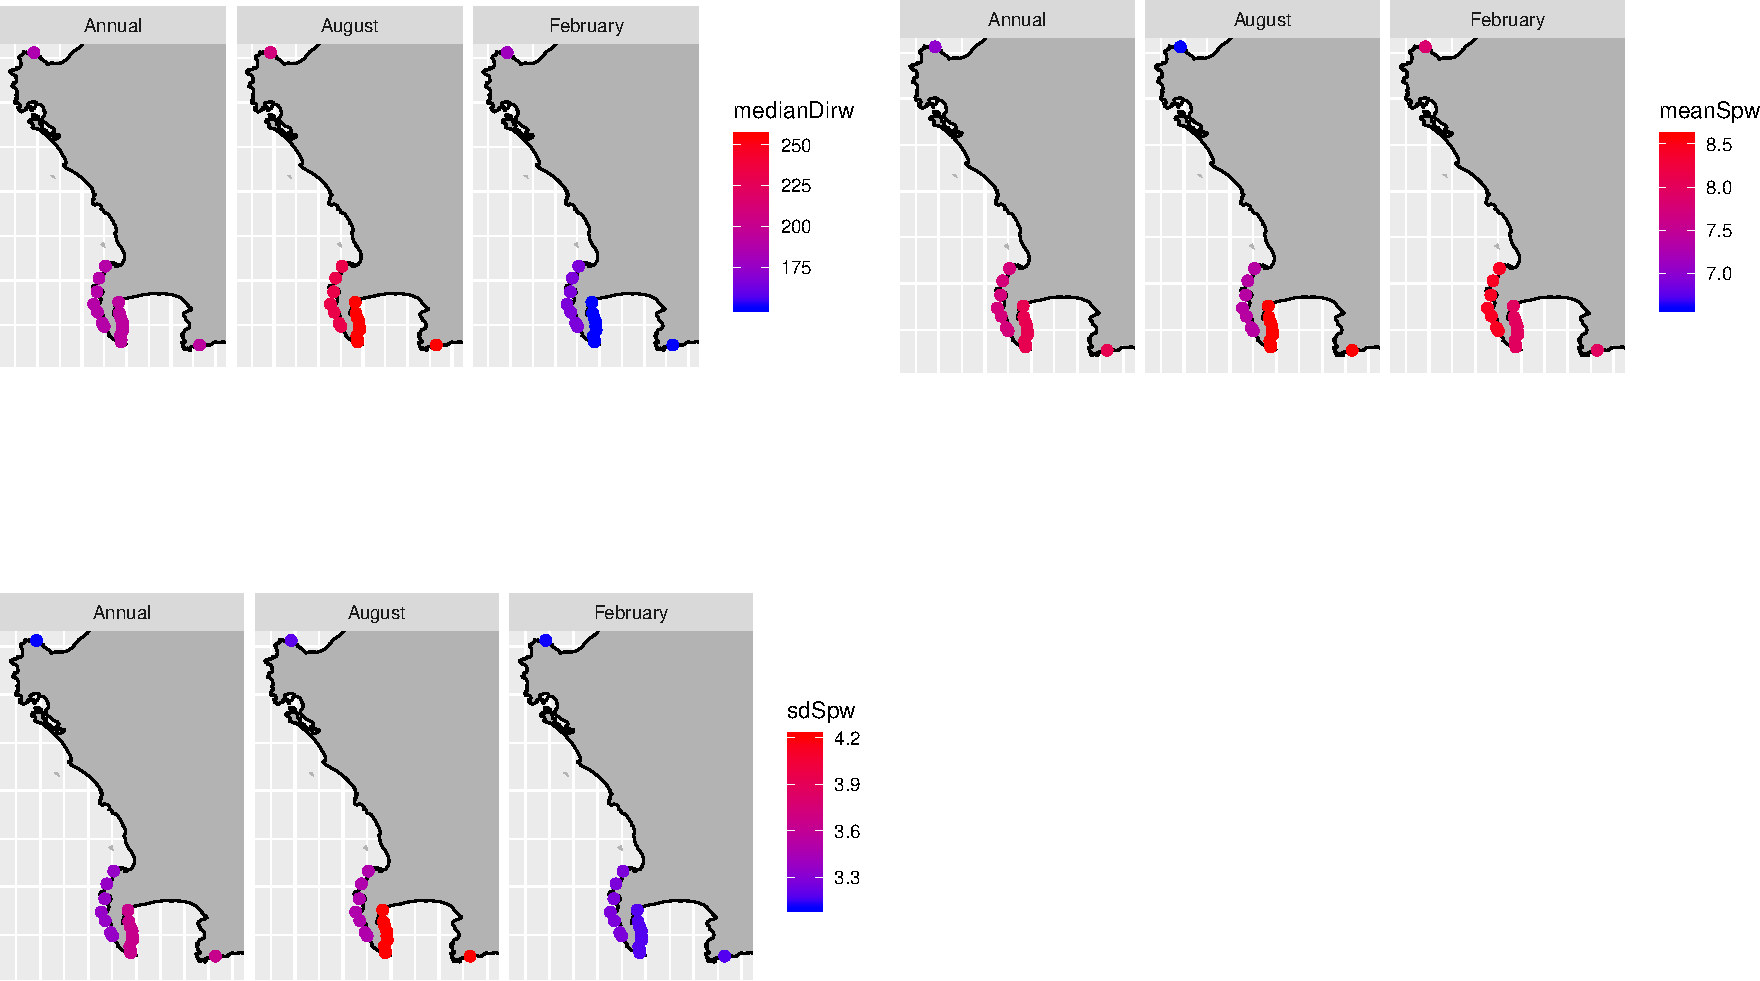
\includegraphics{chapter_2_files/figure-latex/unnamed-chunk-16-1.pdf}
\caption{Wind parameters relative to each morphometric collection site
around the Western Cape coast. These wind parameters include mean and
standard deviation of wind direction (° True north) as well as wind
speed (Meters/ second). Sites are colour-coded by the parameter
statistic provided by the legend. Each wave parameter is also divided
into August (winter), February (summer) and annual means, to visualise
seasonal differences.}
\end{figure}

\hypertarget{morphologies}{%
\subsubsection{Morphologies}\label{morphologies}}

\hypertarget{laminaria-pallida}{%
\paragraph{\texorpdfstring{\emph{Laminaria
pallida}}{Laminaria pallida}}\label{laminaria-pallida}}

Lamina length for laminaria pallida showed no geographical pattern
moving from west to east. Kommetjie, Olifantsbos and Batsata Rock showed
great variability in lamina length, and both Buffels Bay and Betty's Bay
were visually different to Miller's Point and Roman Rock, when comparing
summary data (Fig.8). Lamina thickness showed great variation across
sites, with Baboon Rock, Miller's Point, A-Frame and Roman rock
displaying large lamina thickness, significantly different to the rest
of the sites. Lamina weight was observed to vary for Baboon Rock and
Betty's Bay. Neighbouring sites A-Frame and Roman Rock also showed
visual difference when comparing boxplot summary statistics. An increase
in the number of digits was observed as one moved from Cape Point north
along the western side of False Bay. This ceased at Batstata Rock, which
exhibited significantly less digits compared to the previous site,
Bordjies reef North. Stipe diameter showed some geographical grouping,
with west of Cape Point sites exhibiting larger stipe diameters compared
to False Bay sites.

Stipe diameter decreased as one rounded the point into False Bay, where
a sudden, significant difference was seen between Bordjies reef North
and Batsata Rock. Greater variation of stipe length was observed for
sites outside of False Bay (Kommetjie, Olifantsbos and Betty's Bay).
Baboon Rock, Miller's Point, A-Frame and Roman Rock were again grouped
together exhibiting the lowest stipe lengths, that were all
significantly different to sites found west of Cape Point. Stipe mass
displays similar patterns to stipe length, with larger stipe lengths
west of Cape Point compared to within False Bay. The thallus mass of
\emph{Laminaria pallida} was observed to be greater for sites around
Cape Point, with an observed difference between Batsata Rock and
Bordjies reef North, similar to the number of digit patterns. Larger
total lengths were observed around Cape Point and Betty's Bay, with the
smallest total lengths at sites that exhibited the greatest lamina
thicknesses (Baboon Rock, Miller's Point, A-Frame and Roman Rock).

\begin{figure}
\centering
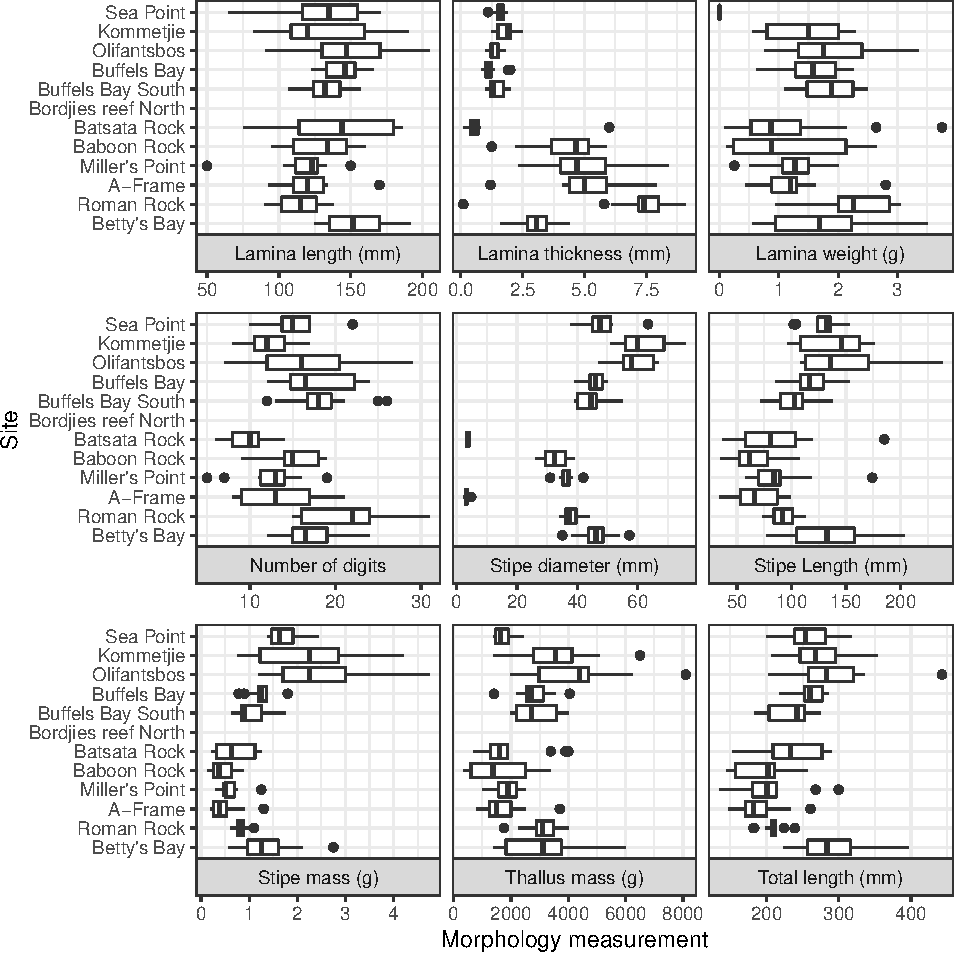
\includegraphics{chapter_2_files/figure-latex/unnamed-chunk-17-1.pdf}
\caption{Boxplots representing the different \emph{Laminaria pallida}
morphometrics measured around the Western Cape coastline, with the
X-axis depicting the specific morphology measured, with units provided.
Boxplots represent the minimum, 25\textsuperscript{th} percentile,
median and 75\textsuperscript{th} percentile of the morphometrics
measured. Interquartile range can be deduced as the different between
the 75\textsuperscript{th} and 25\textsuperscript{th} percentiles, and
dots represent outliers in the data. Sites are ordered sequentially on
the Y-axis by location along the coast. The top site is Sea Point and is
located at the north western boundary, and Betty's Bay as the bottom
site is located at the south eastern boundary, from our sample region.}
\end{figure}

\hypertarget{ecklonia-maxima}{%
\paragraph{\texorpdfstring{\emph{Ecklonia
maxima}}{Ecklonia maxima}}\label{ecklonia-maxima}}

For frond length, frond mass, stipe circumferences, stipe length and
total length of \emph{Ecklonia maxima} morphometrics, we see a gradual
increase in value as one moves south from St.~Helena Bay to Kommetjie
and Soetwater (Fig. 9). Hout Bay, Kommetjie and Soetwater show
similarities in their stipes lengths to Buffels Bay, Batsata Rock and
Betty's Bay, and are significantly different to west of Cape Point
counterpart sites such as Oudekraal and Scarborough. A difference for
the majority of the morphologies are seen between Soetwater and
Scarborough, with significant differences for epiphyte length, frond
length, frond mass, stipe length, stipe mass and total length. A
separation along the same stretch of coast (west of Cape Point) for
stipe mass shows that Hout Bay, Kommetjie and Soetwater are again
significantly different to neighboring west side sites such as Oudekraal
and Scarborough.

\begin{figure}
\centering
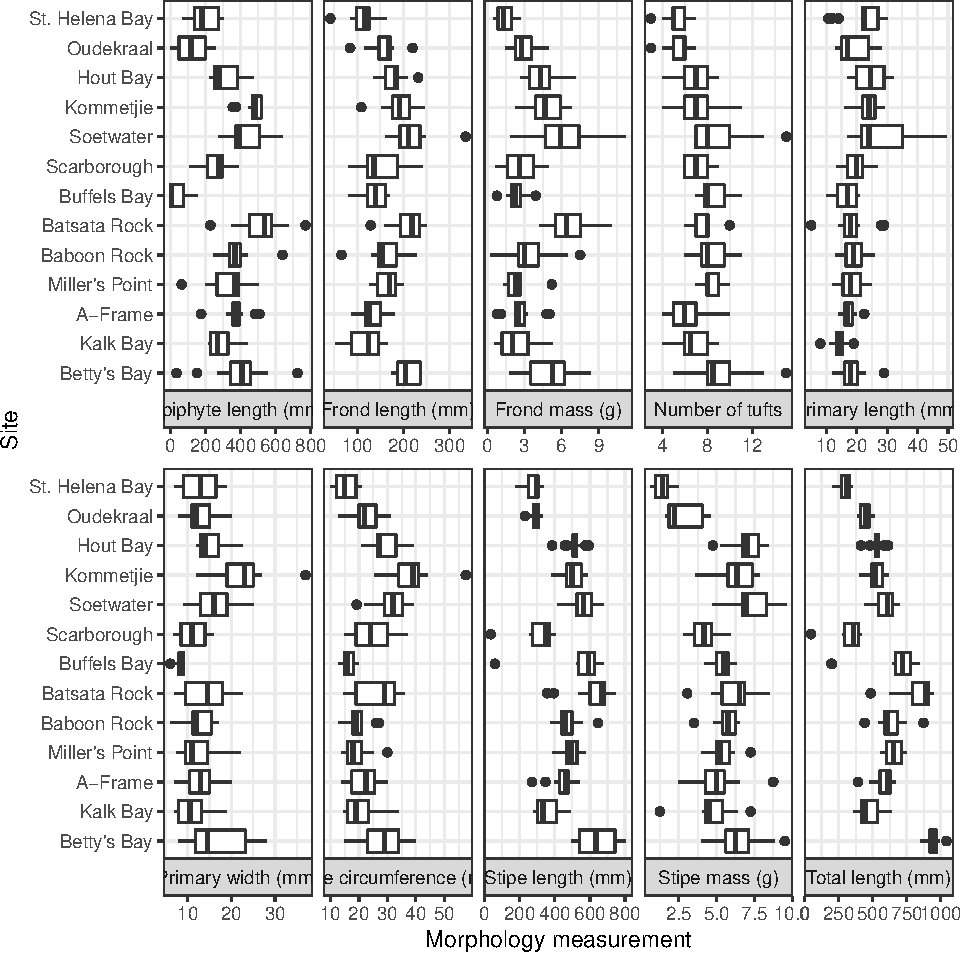
\includegraphics{chapter_2_files/figure-latex/unnamed-chunk-18-1.pdf}
\caption{Boxplots representing the different \emph{Ecklonia maxima}
morphometrics measured around the Western Cape coastline, with the
X-axis depicting the specific morphology measured, with units provided.
Boxplots represent the minimum, 25\textsuperscript{th} percentile,
median and 75\textsuperscript{th} percentile of the morphometrics
measured. Interquartile range can be deduced as the different between
the 75\textsuperscript{th} and 25\textsuperscript{th} percentiles, and
dots represent outliers in the data. Sites are ordered sequentially on
the Y-axis by location along the coast. The top site is St.~Helena Bay
and is located at the north western boundary, and Betty's Bay as the
bottom site is located at the south eastern boundary, from our sample
region.}
\end{figure}

When comparing morphologies bewteen deep and shallow water
\emph{Ecklonia maxima} individuals, clear pattern is seen in certian
morphological characteristics (Fig. 10). These are frond length, frond
mass, primary length, primary width and stipe circumference, and all
show a similar pattern. Significant differences in these morphological
characterstics at Kommetjie and Soetwater are evident, however there are
no significant differences from Buffel's Bay to Kalk Bay.

\begin{figure}
\centering
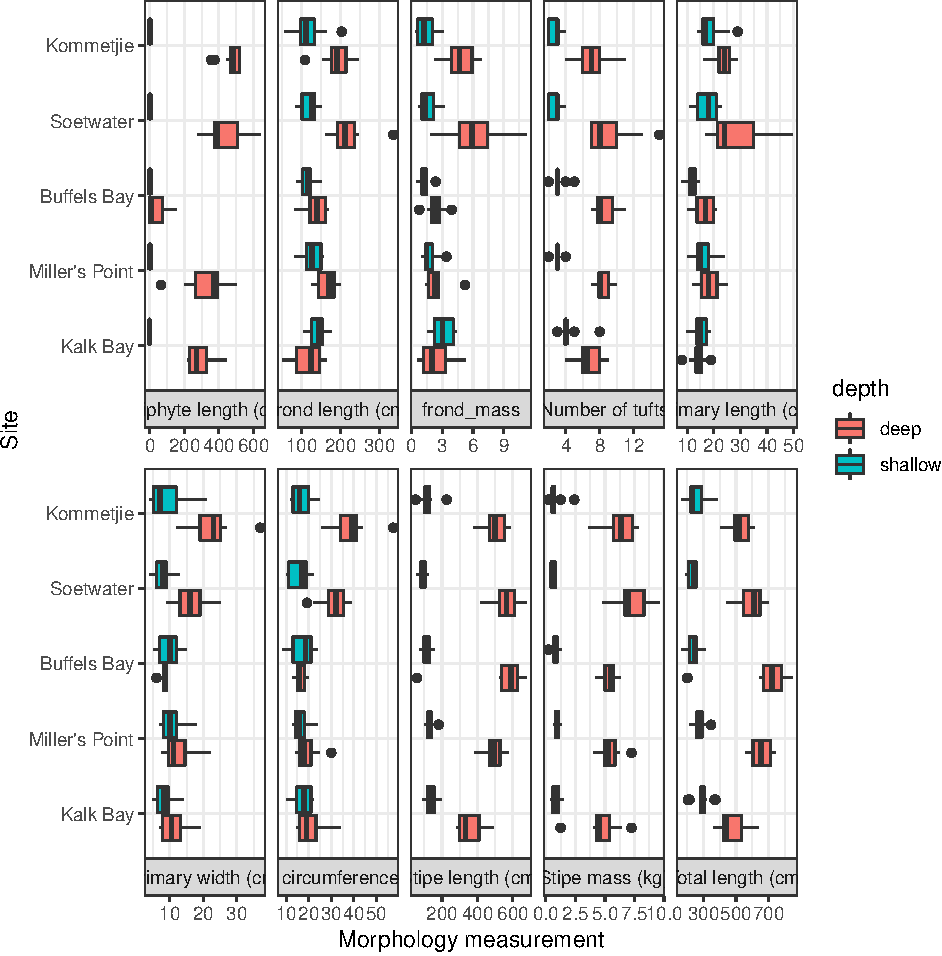
\includegraphics{chapter_2_files/figure-latex/unnamed-chunk-19-1.pdf}
\caption{Boxplots representing the different \emph{Ecklonia maxima}
morphometrics between deep and shallow water sites measured around the
Western Cape coastline, with the X-axis depicting the specific
morphology measured, with units provided. Boxplots represent the
minimum, 25\textsuperscript{th} percentile, median and
75\textsuperscript{th} percentile of the morphometrics measured.
Interquartile range can be deduced as the different between the
75\textsuperscript{th} and 25\textsuperscript{th} percentiles, and dots
represent outliers in the data. Sites are ordered sequentially on the
Y-axis by location along the coast. The top site is St.~Helena Bay and
is located at the north western boundary, and Betty's Bay as the bottom
site is located at the south eastern boundary, from our sample region.}
\end{figure}

\hypertarget{abiotic-correlations}{%
\subsubsection{Abiotic correlations}\label{abiotic-correlations}}

There are various strong correlations within the temperature parameters,
and within the wave parameters on an annual time scale (Fig. 11). SD
Significant wave height (Hs) and mean Hs showed a strong positive
correlate(0.92), as well as SD wave period (Tp) and mean Hs with a
strong negative correlation(-0.9) For SD wind speed and mean wind speed
a strong positive correlation existed (0.967). Minimum and mean
temperatures correlate strongly (0.918), as well as SD wind speed and
median wind direction (0.999). A strong correlation exists between SD
temperature and temperature range (0.942). Median wind direction and
mean wind speed are also correlated well (0.954). We however see no
strong correlations between wave and temperature parameters (Fig 12).

These correlations vary through the three timescales (Annual, August and
February). Although there are no strong correlations between temperature
and wave parameters, we see interesting differences between the seasonal
timescales. The mean temperature and mean wind speed are weakly
correlated in August (0.253)(Fig. 12), but are observed to be more
strongly negatively correlated in February (-0.788)(Fig. 13). The same
is seen for minimum temperature and median wind direction in August
(0.129) compared to February (-0.715).

\begin{figure}
\centering
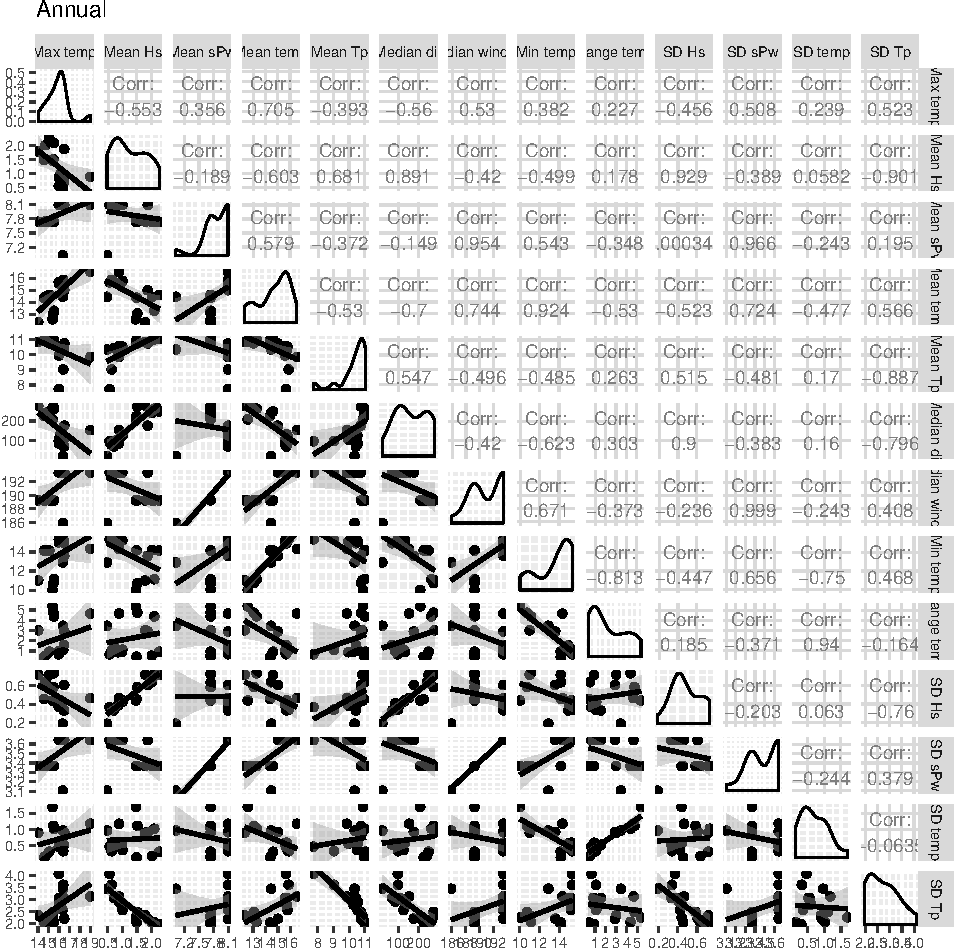
\includegraphics{chapter_2_files/figure-latex/unnamed-chunk-21-1.pdf}
\caption{A correlation graph depicting the relationships that various
temperature and wave parameters share, at an annual timescale. The left
Y-axis as well as bottom X-axis represent the measurements for the
parameters, while the top X-axis and right Y-axis depict the abiotic
parameter name. The top right section of the graph represents
correlation coefficients between abiotic parameters. The bottom left
section provides individual linear regressions between each abiotic
parameter, with a fitted line. Each point of each linear graph
represents a collection site. The diagonal density plots represent the
spread of the data for each abiotic relationship.}
\end{figure}

\begin{figure}
\centering
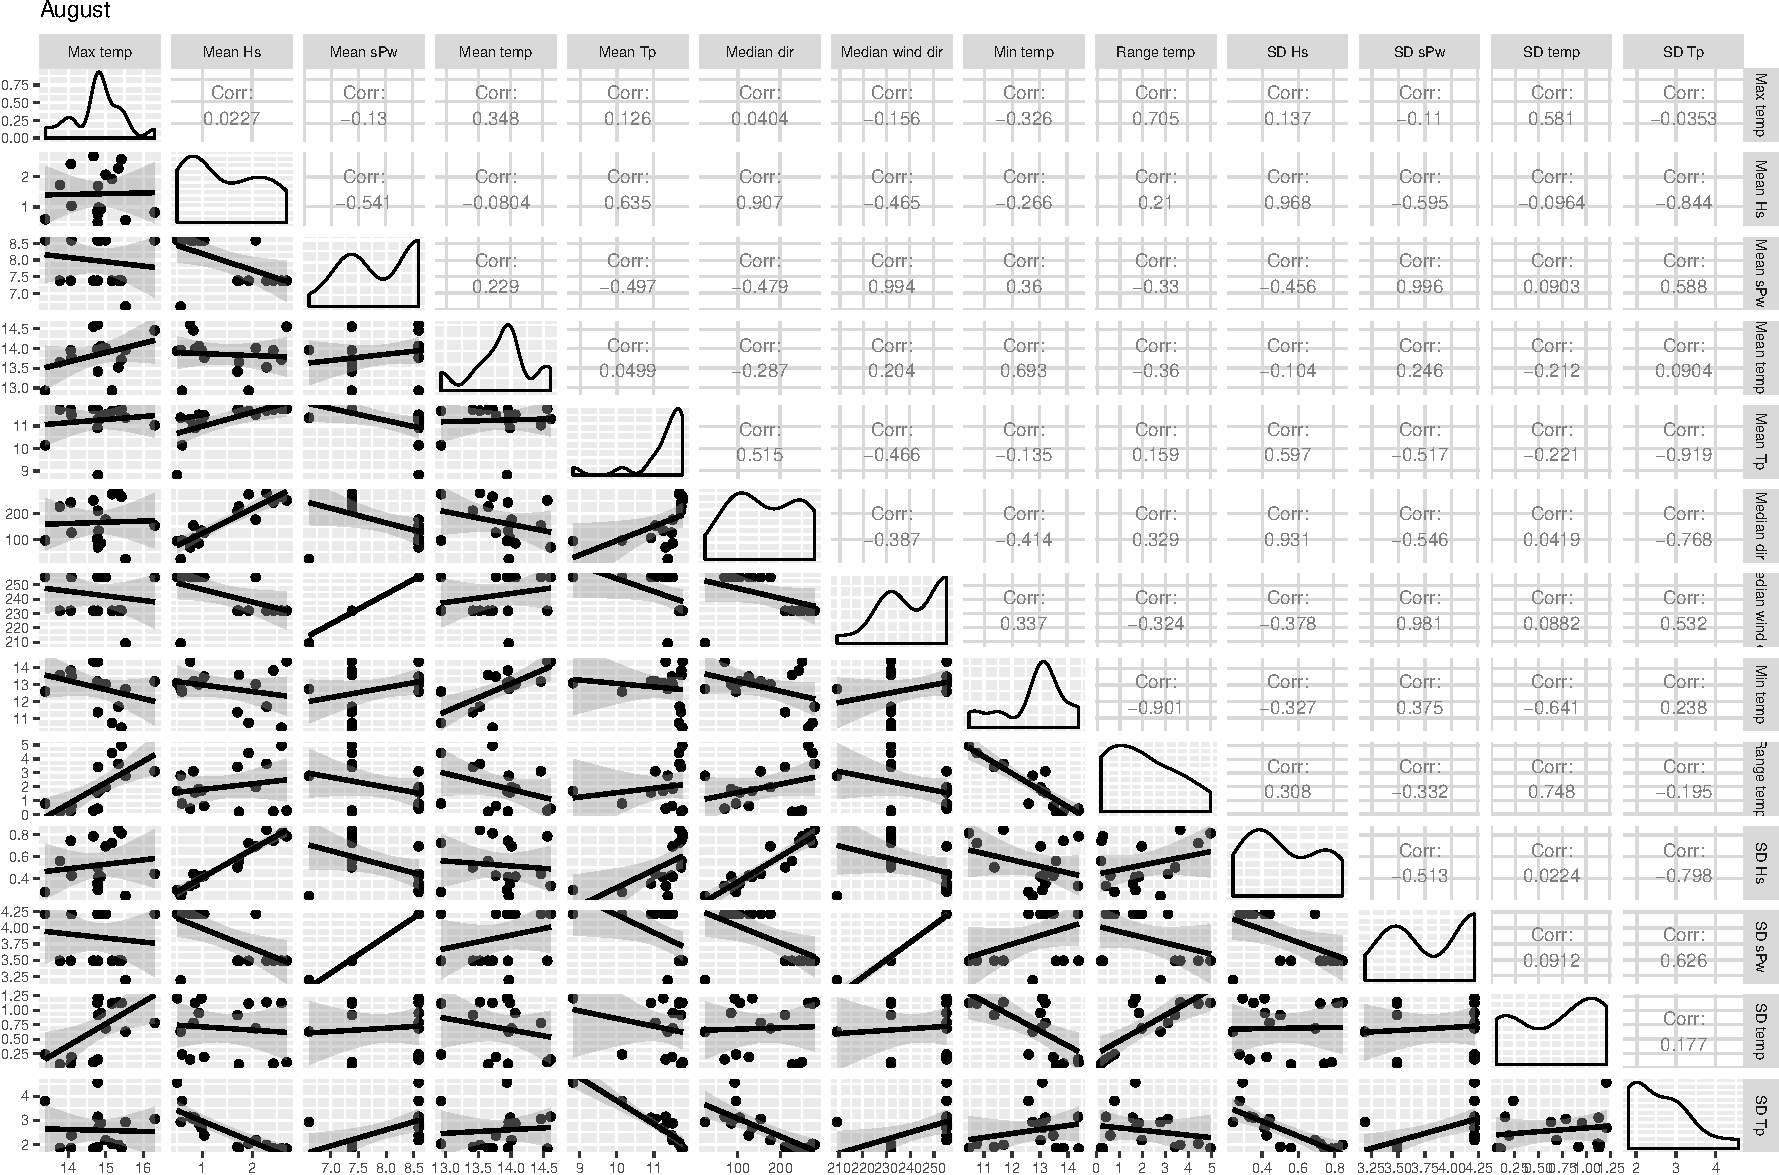
\includegraphics{chapter_2_files/figure-latex/unnamed-chunk-22-1.pdf}
\caption{A correlation graph depicting the relationships that various
temperature and wave parameters share, during August. The left Y-axis as
well as bottom X-axis represent the measurements for the parameters,
while the top X-axis and right Y-axis depict the abiotic parameter name.
The top right section of the graph represents correlation coefficients
between abiotic parameters. The bottom left section provides individual
linear regressions between each abiotic parameter, with a fitted line.
Each point of each linear graph represents a collection site. The
diagonal density plots represent the spread of the data for each abiotic
relationship.}
\end{figure}

\begin{figure}
\centering
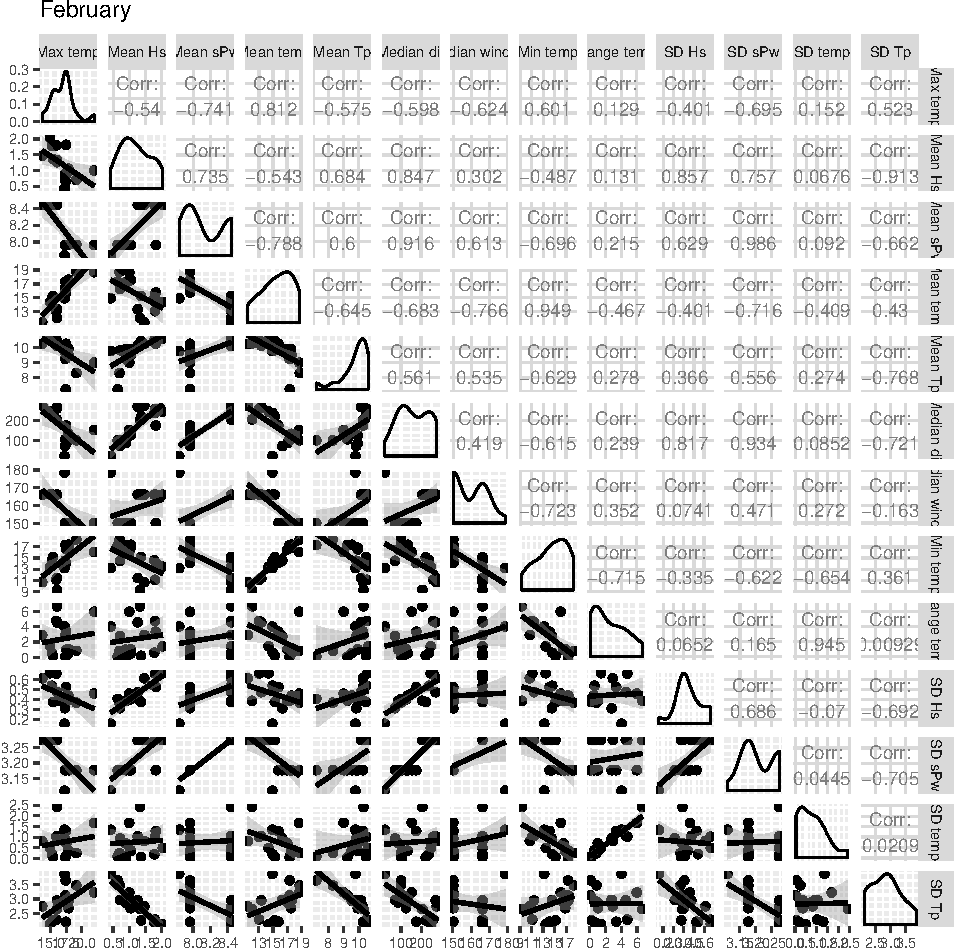
\includegraphics{chapter_2_files/figure-latex/unnamed-chunk-23-1.pdf}
\caption{A correlation graph depicting the relationships that various
temperature and wave parameters share, during February. The left Y-axis
as well as bottom X-axis represent the measurements for the parameters,
while the top X-axis and right Y-axis depict the abiotic parameter name.
The top right section of the graph represents correlation coefficients
between abiotic parameters. The bottom left section provides individual
linear regressions between each abiotic parameter, with a fitted line.
Each point of each linear graph represents a collection site. The
diagonal density plots represent the spread of the data for each abiotic
relationship.}
\end{figure}

\hypertarget{redundancy-analyses}{%
\subsubsection{Redundancy analyses}\label{redundancy-analyses}}

\hypertarget{waves-as-a-driver-of-ecklonia-maxima-morphometrics}{%
\paragraph{\texorpdfstring{Waves as a driver of \emph{Ecklonia maxima}
morphometrics}{Waves as a driver of Ecklonia maxima morphometrics}}\label{waves-as-a-driver-of-ecklonia-maxima-morphometrics}}

The morphometrics of \emph{Ecklonia maxima} were explained more by wave
parameters (75\%), than temperature parameters (66\%), when separate
RDA's were constructed (Fig. 14). The first two axes for wave parameters
driving \emph{Ecklonia maxima} morphology explained 34\% of the
variation. Stipe circumference was positively influenced by both mean
and SD annual significant wave height as well as annual mean wave
direction. There was also a negative influence by annual SD of wave
period and wave direction (which correlate with one another) on stipe
circumference. The primary length of \emph{Ecklonia maxima} was
influenced positively by annual mean wind direction, and negatively
explained by annual SD wind direction.

\begin{figure}
\centering
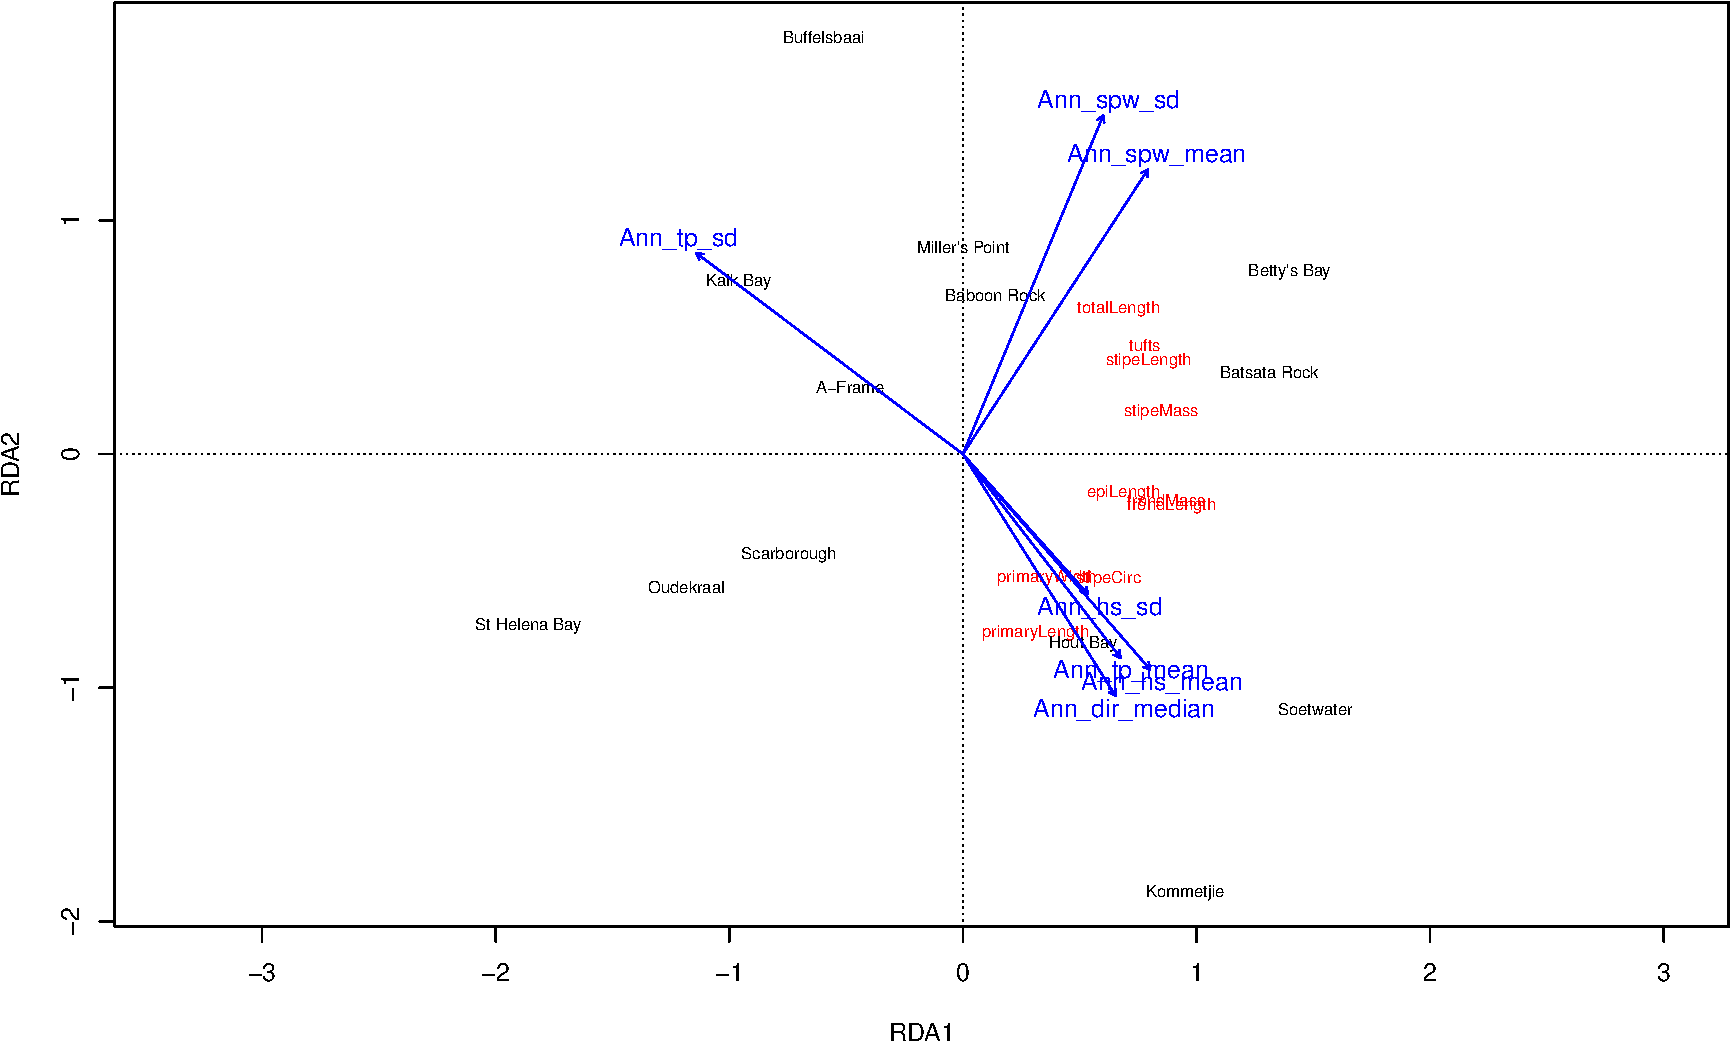
\includegraphics{chapter_2_files/figure-latex/unnamed-chunk-25-1.pdf}
\caption{An RDA, represented by the first two RDA axes, depict the
influence that annual wave parameters have on the morphology of
\emph{Ecklonia maxima} sporophytes. Environmental (explanatory)
variables, in this case annual wave parameters, are represented by blue
vectors extending from the origin. Response variables, in this case
\emph{Ecklonia maxima} morphologies, are representing by red points
ordinated across the plane. Sites are represented in black. The top
X-axis and right Y-axis represent the explanatory variable axes, while
bottom X-axis and left Y-axis represent the response variables axes}
\end{figure}

\hypertarget{temperature-as-a-driver-of-ecklonia-maxima-morphometrics}{%
\paragraph{\texorpdfstring{Temperature as a driver of \emph{Ecklonia
maxima}
morphometrics}{Temperature as a driver of Ecklonia maxima morphometrics}}\label{temperature-as-a-driver-of-ecklonia-maxima-morphometrics}}

Although temperature parameters for \emph{Ecklonia maxima} showed some
influence of the morphometric data, the explanation of morphology was
not strong, with an R\textsuperscript{2} value of 0.662 and a negative
adjusted R\textsuperscript{2} value (-0.138)(Fig. 15). Adjusted
R\textsuperscript{2} values are modified R\textsuperscript{2} values to
include the number predictors in a model. A negative adjusted R squared
values equate to low explanatory power. This is supported by the lack of
relationships between environmental (temperature) and response
(morphology) variables (Fig. 15).

\begin{figure}
\centering
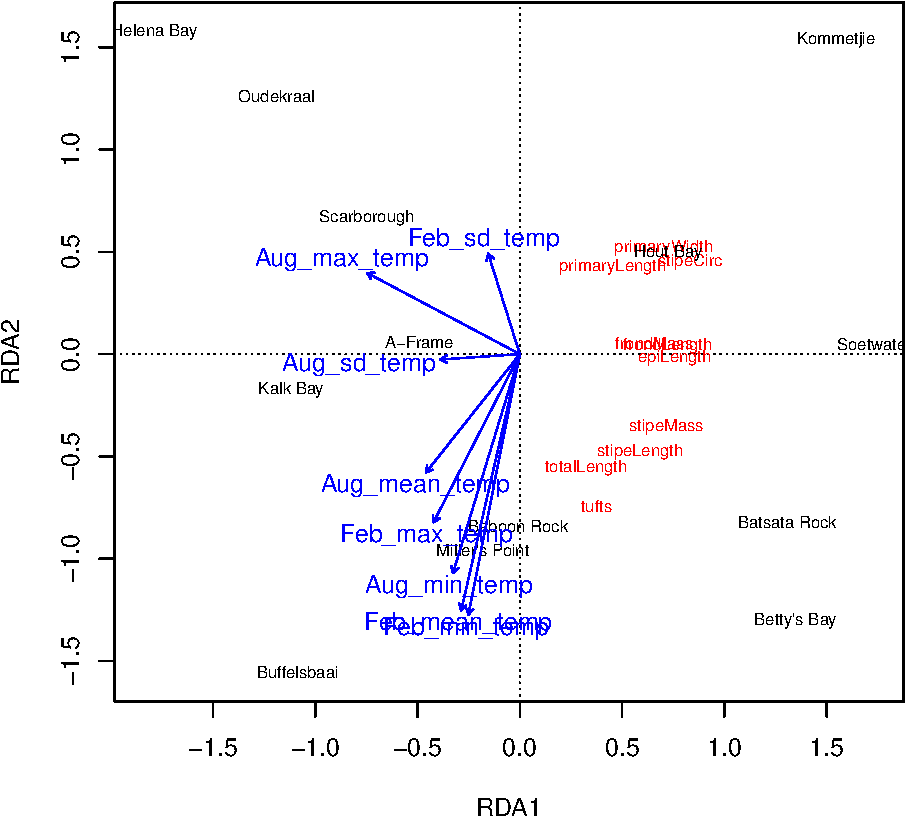
\includegraphics{chapter_2_files/figure-latex/unnamed-chunk-27-1.pdf}
\caption{An RDA, represented by the first two RDA axes, depict the
influence that seasonal temperature parameters have on the morphology of
\emph{Ecklonia maxima} sporophytes. Environmental (explanatory)
variables, in this case seasonal temperature parameters, are represented
by blue vectors extending from the origin. Response variables, in this
case \emph{Ecklonia maxima} morphologies, are representing by red points
ordinated across the plane. Sites are represented in black. The top
X-axis and right Y-axis represent the explanatory variable axes, while
bottom X-axis and left Y-axis represent the response variables axes.}
\end{figure}

\hypertarget{waves-as-a-driver-of-laminaria-pallida-morphometrics}{%
\paragraph{\texorpdfstring{Waves as a driver of \emph{Laminaria pallida}
morphometrics}{Waves as a driver of Laminaria pallida morphometrics}}\label{waves-as-a-driver-of-laminaria-pallida-morphometrics}}

For \emph{Laminaria pallida}, the percentage of explained data by wave
parameters was 89\%, compared to temperature parameters explaining 82\%
(Fig. 16). By using adjusted R\textsuperscript{2} values, the first two
axes for wave parameters driving \emph{Laminaria pallida} morphology
explained 57\% of the variation of morphology in this species. An
increase in annual SD of wave period and wave direction was a strong
influence on lamina thickness of \emph{Laminaria pallida}. Annual mean
wave period (which negatively correlates with both annual SD of wave
period and wave direction) saw a strong positive influence on lamina
length, and a negative influence on lamina thickness. Stipe mass of
\emph{Laminaria pallida} was influenced by annual mean wind direction,
as well as annual mean significant wave height, wave direction and SD of
significant wave height. The Total length of \emph{Laminaria pallida}
specimens were similarly explained by annual mean significant wave
height, wave direction and SD of significant wave height.

\begin{figure}
\centering
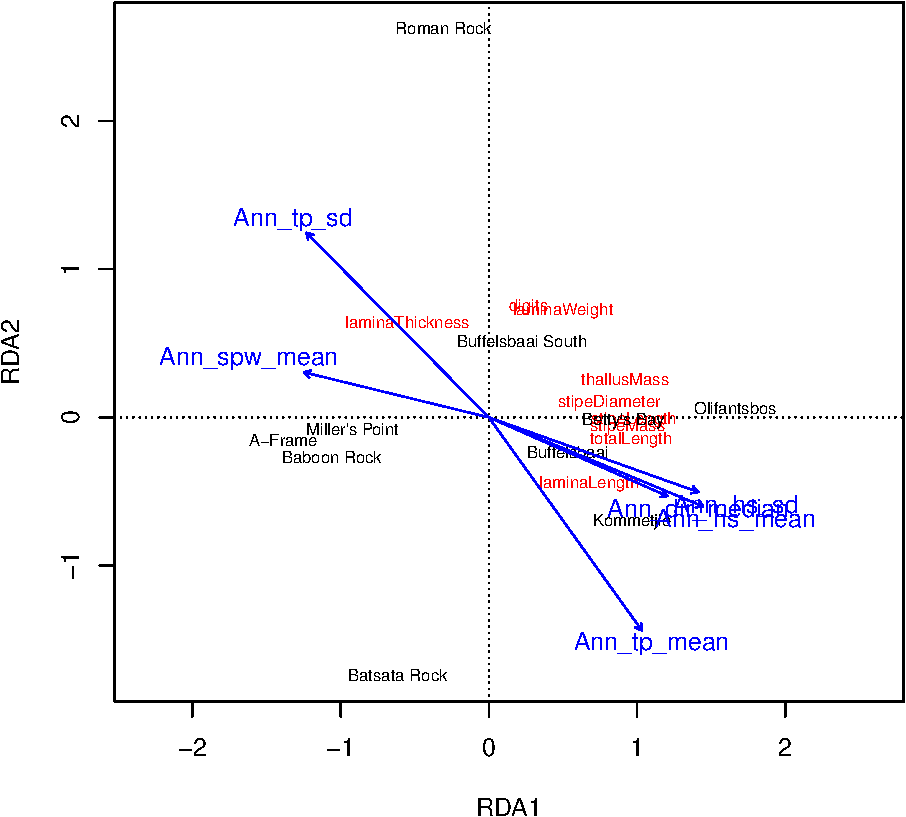
\includegraphics{chapter_2_files/figure-latex/unnamed-chunk-29-1.pdf}
\caption{An RDA, represented by the first two RDA axes, depict the
influence that annual wave parameters have on the morphology of
\emph{Laminaria pallida} sporophytes. Environmental (explanatory)
variables, in this case annual wave parameters, are represented by blue
vectors extending from the origin. Response variables, in this case
\emph{Laminaria pallida} morphologies, are representing by red points
ordinated across the plane. Sites are represented in black. The top
X-axis and right Y-axis represent the explanatory variable axes, while
bottom X-axis and left Y-axis represent the response variables axes.}
\end{figure}

\hypertarget{temperature-as-a-driver-of-laminaria-pallida-morphometrics}{%
\paragraph{\texorpdfstring{Temperature as a driver of \emph{Laminaria
pallida}
morphometrics}{Temperature as a driver of Laminaria pallida morphometrics}}\label{temperature-as-a-driver-of-laminaria-pallida-morphometrics}}

Provided by adjusted R\textsuperscript{2} values, the first two axes of
temperature effect on \emph{Laminaria pallida} morphologies amounted to
only 11\%, but exhibited a stronger influence than on \emph{Ecklonia
maxima} (Fig. 17). The mean and minimum temperatures during February
were observed to negatively influence \emph{Laminaria pallida}
morphologies such as stipe mass, stipe length and stipe diameter, as
well as thallus mass and total length. Maximum august temperatures
however were observed to positively explain stipe diameter of
\emph{Laminaria pallida}.

\begin{figure}
\centering
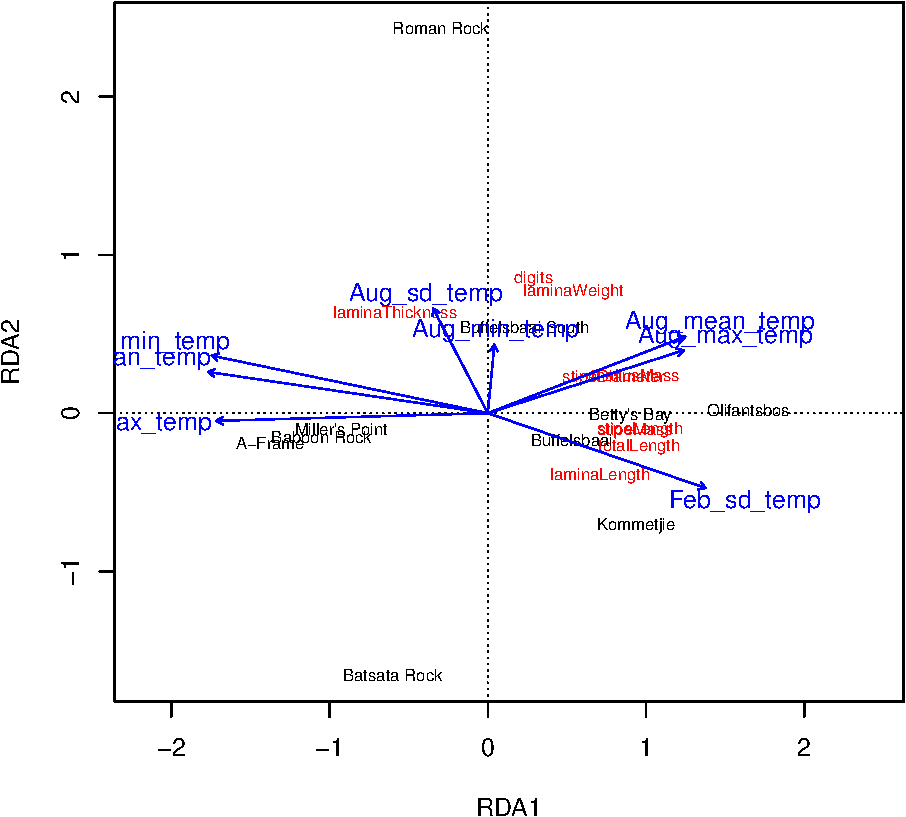
\includegraphics{chapter_2_files/figure-latex/unnamed-chunk-31-1.pdf}
\caption{An RDA, represented by the first two RDA axes, depict the
influence that seasonal temperature parameters have on the morphology of
\emph{Laminaria pallida} sporophytes. Environmental (explanatory)
variables, in this case seasonal temperature parameters, are represented
by blue vectors extending from the origin. Response variables, in this
case \emph{Laminaria pallida} morphologies, are representing by red
points ordinated across the plane. Sites are represented in black. The
top X-axis and right Y-axis represent the explanatory variable axes,
while bottom X-axis and left Y-axis represent the response variables
axes.}
\end{figure}

\newpage

\hypertarget{discussion}{%
\subsection{Discussion}\label{discussion}}

Kelps, in particular brown seaweeds, are robust and resilient organisms
that have been shown to adapt their morphology to suit local
environmental conditions (refs.). Wave exposure has been shown to be the
main driver of morphological variation in brown seaweeds as a strategy
to reduce drag and ultimately dislodgement (refs.). Although wave
exposure is regarded as an important abiotic variable that drives kelp
morphology, it does not act independently \{AJS: of what?\}. For
instance, a study by Wernberg and Thomsen (2005) investigated the effect
of wave exposure on the morphology of \emph{Ecklonia radiata} of six
locations along 1100 km of the southwest Australian coastline. The
authors concluded that wave exposure was the main driver of kelp
morphological adaptation in the study; however, they also noted the
variation in morphology between sites was not consistent and concluded
that wave parameters may play different roles in determining kelp
morphology \{AJS: What does this mean?\}. The results from this current
study confirm the idea that kelp morphology is driven by specific wave
parameters, particularly significant wave height, wave period and wave
direction \{AJS: what about?\}.

Seasonal variations in significant wave height (Hs), wave period and
wave direction were observed from the data. The direction of swell
swings to the south west in winter, generated by strong low pressures
that originate from the southern ocean (Reason et al. 2006). These
swells were found to correlate with increased wave period (Tp), wave
direction and Hs. False Bay is therefore shielded by these south
westerly swells by the Cape Peninsula (Shipley 1964). In summer, these
swells rotate anticlockwise and are able to enter False Bay, providing
an explanation for increased variability of Hs and Tp. However, changing
winds may also be influencing waves generated within False Bay. As seen
in Figure 1 the summer and winter swells are relativley constant in
terms of direction adn this may be driving the waves locally (I am still
looking for the report where Christo cites this). The wind speed and
wind direction support the presence of upwelling in summer, where
southerly winds blow parallel to the coast and trigger upwelling (Field
et al. 1980b). This is supported by the decreased in temperature in
summer, specifically along the west side of Cape Point. We however see a
differentiation of median wind directions in summer, with the western
coast of False Bay experiencing south easterly winds, compared to the
west side of Cape Point experiencing south westerly winds. It is
hypothesised that the topography and elevation along the Cape Peninsula
channels, shields winds along the strip of land. This is however absent
in winter, where strong northerly winds are experiences from St.~Helena
Bay to Betty's Bay (Field et al. 1980b). St.~Helena bay experiences
decreased median wave directions, and is protected by a headland,
similar to the sites found along the western side of False Bay, that are
shielded by the Cape Peninsula. There is however increased variability
in the wave direction from both False Bay sites and St.~Helena Bay,
which is encouraged by refraction of waves.

Morphological adaptation due to water motion may manifest itself in a
number of ways to high wave energy environments. For instance, reduction
of blade thickness, blade elongation, increase of stipe length, and
stipe circumference increase and force of attachment. Although this
study did not measure force of attachment, other morphological responses
to wave parameters was evident. An increase in mean annual wave period
saw an increase of lamina length of \emph{Laminaria pallida}, but a
decrease in lamina thickness. By decreasing the thickness of the lamina,
and increasing the length of the lamina (directly increasing surface
area), a larger more flexible kelp can survive in environments with
greater wave period. Increased thickness of cortical tissues within the
lamina aid photosynthetic ability ({\textbf{???}}), however increased
wave exposure deceases the boundary diffusion layer ({\textbf{???}},
{\textbf{???}}). Therefore \emph{Laminaria pallida} in increased wave
period sites may be able to reduce the need for thick lamina for
photosynthesis, as the increased wave period provide longer wave events,
which decreases the diffusion boundary layer and allow easier nutrient
uptake. Conversely we see that sites with reduced wave height and wave
period, such as Baboon Rock, Miller's Point, A-Frame and Roman Rock
displayed the greatest lamina thickness, with better photosynthetic
ability, for \emph{Laminaria pallida}. Pace ({\textbf{???}}) however
studied the effect of wave exposure on \emph{Macrocystis pyrifera}
morphologies, and found that lamina thickness had a strong positive
relationship with wave exposure. This may be species specific, with
\emph{Macrocystis pyrifera} attaining larger sizes, but with
incomparable stipe and lamina morphologies to \emph{Ecklonia maxima} and
\emph{Laminaria pallida}.

Lamina thickness showed positive correlation with annual SD wave period.
Although this variable may just negatively correlate with annual mean
wave period, another reason may exist. The greatest variation of wave
period and wave direction occurs in August along the western side of
False Bay. Kelps at these sites may have developed thicker lamina, with
a possible strategy of maximising photosynthesis at the expense of maybe
being dislodged through rare increased wave energy events. The
`spreading out' of the lamina may also suggest a `go with the flow'
tactic, to reduce breaking by being less stiff (Friedland and Denny
1995). Denny et al. (1997) explored the stress forces that wave period
played on \emph{Nereocystis luetkeana} by exposing various kelp plant
sizes to a range of wave period that would be found in coastal
environments. Results showed that for shorter kelps (smaller stipe
lengths), the maximum stress on a plant occurs at 10s wave periods, but
only at 5.5s for larger kelps that are similar in length to the water
depth. Similar results were observed for kelps with larger blades, with
maximal stress forces occurring at approximately 8s, compared to a
stress ratio of only 0.4 at 16s wave periods.

Mean annual significant wave height (Hs) was observed to influence
\emph{Ecklonia maxima} stipe circumference, with increased stipe
circumference at larger Hs. An increase in Hs saw greater wave actions
as waves are larger, as well as greater wave periods that are positively
correlated with Hs. An increase in stipe circumference provides
\emph{Ecklonia maxima} with a more rigid structure to withstand the
onslaught of waves. These greater stipe circumferences of \emph{Ecklonia
maxima} were observed at west side sites such as Soetwater and
Kommetjie. While these sites experience increased Hs, they also are
subject to seasonal upwelling events ({\textbf{???}}), that bring with
it cold clean water. \emph{Ecklonia maxima} are thought to be influenced
greatly by light attenuation (Rothman et al. 2017), and thus have
developed increased (stronger) stipe circumferences to be able to cope
in large Hs environments, to access cleaner, nutrient-filled water. The
same patterns are observed in \emph{Laminaria pallida} morphologies,
that display increased stipe diameters at Soetwater and Kommetjie as
well. This increase in stipe diameter correlates with stipe mass of
\emph{Laminaria pallida}, providing evidence that this species has
developed thicker, strong stipes to persist in this region. Denny et
al.~(1997) found that the stress ratio decreased as stipe lengths
increases, in a fixed depth. Therefore adult \emph{Ecklonia maxima}
sporophytes would experience a lower stress ratio compared to adult
\emph{Laminaria pallida} sporophytes in the same environment, where
\emph{Laminaria pallida} is often a subsurface species to \emph{Ecklonia
maxima}. Stipe circumference for \emph{Ecklonia maxima} were explained
by annual wave direction. For \emph{Ecklonia maxima}, the sporophytes
may be producing stipes that have a greater circumference to cope with
increased wave energy. The west side of the peninsula is more exposed to
significant wave heights during winter due to the direction of swell,
while other sites such as Betty's Bay and Basata rock are more protected
due to their location along the coast and the presence of headlands
which refract wave parameters.

Temperature parameters were not found to be a significant driver of kelp
morphology in this study. Although temperature plays an important role
in distribution of kelp and physiological functioning of adults and
gametophytes, there is little evidence that temperature is a driver of
morphological variation in kelps. Although turbidity is not a direct
wave or temperature parameter, turbidity is influence by various abiotic
variables. Increased swells around sandy beaches increase sedimentation
and turbidity ({\textbf{???}}), however wind direction and speed can
encourage upwelling, with brings to the surface cold, clean,
nutrient-rich water ({\textbf{???}}). Increased wind speed at sites
along the west side of the peninsula in a southerly direction trigger
upwelling events ({\textbf{???}}). We however see a lack of upwelling
events for sites such as Betty's Bay and Batsata Rock. These two sites
display \emph{Ecklonia maxima} sporophytes with the largest total
lengths, as well as Betty's Bay displaying the largest total length of
\emph{Laminaria pallida} sporophytes. The effect of depth on stipe
length is regarded as insignificant in this study as all kelp were
sampled at similar depths. Stipe elongation has been shown to be a
morphological adaptation in wave exposed environment, as a longer kelp
has time to extend back and forth in swell reducing the tension on the
holdfast. Stipe lengths of \emph{Ecklonia maxima} from Kommetjie, Hout
Bay and Soetwater are similar to Batsata rock and Betty's Bay, but
differs to west side neighbours such as Oudekraal and Scarborough.
Oudekraal and Scarborough experience more variability in wave direction,
however they are observed to experience smaller annual mean significant
wave heights, when compared to Kommetjie, Hout Bay, Soetwater, as well
as Batsata Rock and Betty's Bay. Friedland and Denny (1995) found that
longer kelps were able to reduce drag and tension as the sinusoidal
displacement of most waves would not `stretch' a kelp out long enough
before falling. The ability to grow longer stipes would provide the kelp
with a structure that could surpass most wave heights without the risk
of dislodgement.

\hypertarget{conclusion}{%
\subsection{Conclusion}\label{conclusion}}

(More to add here but I wanted to add it so long) Mechanical dislodgment
through hydrological stress is the main source on mortality for kelp,
and previous research has shown that wave exposure is the main driver of
kelp morphology. Therefore, morphological adaptation is the main
strategy to reduce drag and ultimately dislodgement in hydrological
stressful environments. The results from this study support previous
findings, and shows that particular wave parameters (significant wave
height and median wave direction) act more strongly in driving kelp
morphological plasticity.

\hypertarget{references}{%
\section*{References}\label{references}}
\addcontentsline{toc}{section}{References}

\hypertarget{refs}{}
\leavevmode\hypertarget{ref-Anderson1997}{}%
Anderson, R. J. et al. 1997. Holdfasts of adult kelp Ecklonia maxima
provide refuges from grazing for recruitment of juvenile kelps. - Marine
Ecology Progress Series 159: 265--273.

\leavevmode\hypertarget{ref-DeBettignies2013}{}%
Bettignies, T. de et al. 2013. Size, not morphology, determines
hydrodynamic performance of a kelp during peak flow. - Marine Biology in
press.

\leavevmode\hypertarget{ref-Bologna1993}{}%
Bologna, P. and Steneck, R. S. 1993. Kelp beds as habitat for American
lobster Homarus americanus. - Marine \ldots{} in press.

\leavevmode\hypertarget{ref-Bolton2010}{}%
Bolton, J. J. 2010. The biogeography of kelps (Laminariales,
Phaeophyceae): A global analysis with new insights from recent advances
in molecular phylogenetics. - Helgoland Marine Research 64: 263--279.

\leavevmode\hypertarget{ref-Bolton1985a}{}%
Bolton, J. J. and Levitt, G. J. 1985. Light and temperature requirements
for growth and reproduction in gametophytes of Ecklonia maxima
(Alariaceae: Laminariales). - Marine Biology 87: 131--135.

\leavevmode\hypertarget{ref-Bolton1987}{}%
Bolton, J. J. and Anderson, R. J. 1987. Temperature tolerances of two
southern African Ecklonia species (Alariaceae: Laminariales) and of
hybrids between them. - Marine Biology 96: 293--297.

\leavevmode\hypertarget{ref-Bolton2012}{}%
Bolton, J. J. et al. 2012. South African kelp moving eastwards: the
discovery of Ecklonia maxima (Osbeck) Papenfuss at De Hoop Nature
Reserve on the south coast of South Africa. - African Journal of Marine
Science 34: 147--151.

\leavevmode\hypertarget{ref-Bustamante1996}{}%
Bustamante, R. H. and Branch, G. M. 1996. The dependence of intertidal
consumers on kelp-derived organic matter on the west coast of South
Africa. - Journal of Experimental Marine Biology and Ecology 196: 1--28.

\leavevmode\hypertarget{ref-Cousens1982}{}%
Cousens, R. 1982. The Effect of Exposure to Wave Action on the
Morphology and Pigmentation of Ascophyllum nodosum (L.) Le Jolis in
South-Eastern Canada. - Bontanica Marina XXV: 191--195.

\leavevmode\hypertarget{ref-Dayton1999}{}%
Dayton, P. K. et al. 1999. Temporal and spatial patterns of kelp
demography: The role of Oceanographic climate. - Ecological Monographs
69: 219--250.

\leavevmode\hypertarget{ref-Denny1997}{}%
Denny, M. et al. 1997. Flow and Flexibility: II. THE ROLES OF SIZE AND
SHAPE IN DETERMINING WAVE FORCES ON THE BULL KELP NEREOCYSTIS LUETKEANA
MARK. - Journal of Experimental Biology 200: 3165--3183.

\leavevmode\hypertarget{ref-Duggins2003}{}%
Duggins, D. O. et al. 2003. Population, morphometric and biomechanical
studies of three understory kelps along a hydrodynamic gradient. -
Marine Ecology Progress Series 265: 57--76.

\leavevmode\hypertarget{ref-Field1980b}{}%
Field, J. G. et al. 1980a. Variation in Structure and Biomass of Kelp
Communities Along the South-West Cape Coast. - Transactions of the Royal
Society of South Africa 44: 145--203.

\leavevmode\hypertarget{ref-Field1980a}{}%
Field, J. G. et al. 1980b. Upwelling in a nearshore marine ecosystem and
its biological implications. - Estuarine and Coastal Marine Science 11:
133--150.

\leavevmode\hypertarget{ref-FowlerWalker2006}{}%
Fowler-Walker, M. J. et al. 2006. Differences in kelp morphology between
wave sheltered and exposed localities: Morphologically plastic or fixed
traits? - Marine Biology 148: 755--767.

\leavevmode\hypertarget{ref-Friedland1995}{}%
Friedland, M. T. and Denny, M. W. 1995. Surviving hydrodynamic forces in
a wave-swept environment: consequences of morphology in the feather boa
kelp, Egregia menziesii (Turner). - Journal of Experimental Marine
Biology and \ldots{} in press.

\leavevmode\hypertarget{ref-Gaines1987}{}%
Gaines, S. D. and Roughgarden, J. 1987. Fish in offshore kelp forests
affect recruitment to intertidal barnacle populations. - Science 235:
479--481.

\leavevmode\hypertarget{ref-Graham2007}{}%
Graham, M. H. et al. 2007. Global Ecology of the Giant Kelp Macrocystis
: From Ecotypes To Ecosystems. - Oceanography and Marine Biology 45:
39--88.

\leavevmode\hypertarget{ref-Levin1994}{}%
Levin, P. S. 1994. Fine-scale temporal variation in recruitment of a
temperate demersal fish: the importance of settlement versus
post-settlement loss. - Oecologia 97: 124--133.

\leavevmode\hypertarget{ref-Luning1990}{}%
Lüning, K. 1990. Seaweeds: their environment, biogeography, and
ecophysiology (C Yarish and H Kurkman, Eds.). in press.

\leavevmode\hypertarget{ref-Mann1973}{}%
Mann, K. H. 1973. Seaweeds: Their Productivity and Strategy for Growth.
- Science 182: 975--981.

\leavevmode\hypertarget{ref-Mann1982}{}%
Mann, K. H. 1982. Ecology of Coastal Waters: A Systems Approach. in
press.

\leavevmode\hypertarget{ref-Molloy1996}{}%
Molloy, F. J. and Bolton, J. J. 1996. The effects of wave exposure and
depth on the morphology of inshore populations of the Namibian kelp,
Laminaria schinzii Foslie. - Botanica Marina 39: 525--531.

\leavevmode\hypertarget{ref-moss1948}{}%
Moss, B. 1948. Studies in the genus Fucus: I. on the structure and
chemical composition of Fucus vesiculosus from three Scottish
localities. - Annals of Botany 12: 267--279.

\leavevmode\hypertarget{ref-Norderhaug2012}{}%
Norderhaug, K. M. et al. 2012. Does the diversity of kelp forest
macrofauna increase with wave exposure? - Journal of Sea Research 69:
36--42.

\leavevmode\hypertarget{ref-pedersen2012a}{}%
Pedersen, M. F. and Nejrup, L. B. 2012. Effects of wave exposure on
population structure, demography, biomass and productivity of the kelp
Laminaria hyperborea. - Marine Ecology Progress Series 451: 45--60.

\leavevmode\hypertarget{ref-Probyn1985}{}%
Probyn, T. and McQuaid, C. 1985. In-situ measurements of nitrogenous
nutrient uptake by kelp (Ecklonia maxima) and phytoplankton in a
nitrate-rich upwelling environment. - Marine Biology 88: 149--154.

\leavevmode\hypertarget{ref-Reason2006}{}%
Reason, C. J. C. et al. 2006. Seasonal to decadal prediction of southern
African climate and its links with variability of the Atlantic ocean. -
Bulletin of the American Meteorological Society 87: 941--955.

\leavevmode\hypertarget{ref-Rothman2017}{}%
Rothman, M. D. et al. 2017. Geographical variation in morphology of the
two dominant kelp species, Ecklonia maxima and Laminaria pallida
(Phaeophyceae, Laminariales), on the west coast of Southern Africa. -
Journal of Applied Phycology 29: 2627--2639.

\leavevmode\hypertarget{ref-Santelices2007}{}%
Santelices, B. 2007. The discovery of kelp forests in deep-water
habitats of tropical regions. - Proceedings of the National Academy of
Sciences 104: 19163--19164.

\leavevmode\hypertarget{ref-Shipley1964}{}%
Shipley, A. 1964. Some aspects of wave refraction in False Bay. - South
African Journal of Science 60: 115--120.

\leavevmode\hypertarget{ref-Smit2013}{}%
Smit, A. J. et al. 2013. A coastal seawater temperature dataset for
biogeographical studies: Large biases between in situ and
remotely-sensed data sets around the coast of South Africa. - PLoS ONE
in press.

\leavevmode\hypertarget{ref-Stegenga1997}{}%
Stegenga, H. et al. 1997. Seaweeds of the South African west coast. -
Contributions of the Bolus Herbarium 18: 3--637.

\leavevmode\hypertarget{ref-Steneck2002}{}%
Steneck, R. S. et al. 2002. Kelp forest ecosystems: biodiversity,
stability, resilience and future. - Environmental Conservation 29:
436--459.

\leavevmode\hypertarget{ref-Sundblad2014}{}%
Sundblad, G. et al. 2014. Comparing the ecological relevance of four
wave exposure models. - Estuarine, Coastal and Shelf Science 140: 7--13.

\leavevmode\hypertarget{ref-Veitch2018}{}%
Veitch, J. et al. 2018. 'The Cape Point wave record and the role of
large-scale modes of climate variability'. - Reprint submitted to the
Journal of Marine Systems: 131--135.

\leavevmode\hypertarget{ref-Velimirov1977}{}%
Velimirov, B. et al. 1977. The ecology of kelp bed communities in the
Benguela upwelling system - Analysis of biomass and spatial
distribution. - Helgoländer Wissenschaftliche Meeresuntersuchungen 30:
495--518.

\leavevmode\hypertarget{ref-Wernberg2005}{}%
Wernberg, T. and Thomsen, M. S. 2005. The effect of wave exposure on the
morphology of Ecklonia radiata. - Aquatic Botany 83: 61--70.

\leavevmode\hypertarget{ref-Zimmerman1984}{}%
Zimmerman, R. C. and Kremer, J. N. 1984. Episodic nutrient supply to a
kelp forest ecosystem in Southern California. - Journal of Marine
Research 42: 591--604.

\end{document}
